\documentclass[a4paper, 11pt, notitlepage]{article}

%\usepackage{babel}
\usepackage[utf8]{inputenc}
\usepackage[T1]{fontenc, url}
\usepackage{textcomp}
\usepackage{amsmath, amssymb}
\usepackage{amsbsy, amsfonts}
\usepackage{graphicx, color}
\usepackage{parskip}
\usepackage{framed}
\usepackage{amsmath}
\usepackage{xcolor}
\usepackage{multicol}
\usepackage{url}
\usepackage{flafter}
\usepackage{caption}

%\DeclareCaptionLabelSeparator{colon}{. }
\renewcommand{\captionfont}{\sffamily}
\renewcommand{\captionlabelfont}{\bf\sffamily}
\setlength{\captionmargin}{40pt}

\usepackage{geometry}
\geometry{headheight=0.01mm}
\geometry{top=24mm, bottom=29mm, left=39mm, right=39mm}

\renewcommand{\arraystretch}{2}
\setlength{\tabcolsep}{10pt}
\makeatletter
\renewcommand*\env@matrix[1][*\c@MaxMatrixCols c]{%
  \hskip -\arraycolsep
  \let\@ifnextchar\new@ifnextchar
  \array{#1}}
%
% Parametere for inkludering av kode fra fil
%
\usepackage{listings}

\DeclareMathAlphabet{\mathbfit}{OML}{cmm}{b}{it}

\definecolor{javared}{rgb}{0.6,0,0} % for strings
\definecolor{javagreen}{rgb}{0.25,0.5,0.35} % comments
\definecolor{javapurple}{rgb}{0.5,0,0.35} % keywords
\definecolor{javadocblue}{rgb}{0.25,0.35,0.75} % javadoc

\lstset{language=python,
basicstyle=\ttfamily\scriptsize,
keywordstyle=\color{javapurple},%\bfseries,
stringstyle=\color{javared},
commentstyle=\color{javagreen},
morecomment=[s][\color{javadocblue}]{/**}{*/},
% numbers=left,
% numberstyle=\tiny\color{black},
stepnumber=2,
numbersep=10pt,
tabsize=4,
showspaces=false,
captionpos=b,
showstringspaces=false,
frame= single,
breaklines=true}
%
% Definering av egne kommandoer og miljøer
%
\newcommand{\dd}[1]{\ \text{d}#1}
\newcommand{\f}[2]{\frac{#1}{#2}} 
\newcommand{\beq}{\begin{equation}}
\newcommand{\eeq}{\end{equation}}
\newcommand{\bra}[1]{\langle #1|}
\newcommand{\ket}[1]{|#1 \rangle}
\newcommand{\braket}[2]{\langle #1 | #2 \rangle}
\newcommand{\braup}[1]{\langle #1 \left|\uparrow\rangle\right.}
\newcommand{\bradown}[1]{\langle #1 \left|\downarrow\rangle\right.}
\newcommand{\av}[1]{\left| #1 \right|}
\newcommand{\op}[1]{\hat{#1}}
\newcommand{\braopket}[3]{\langle #1 | {#2} | #3 \rangle}
\newcommand{\ketbra}[2]{\ket{#1}\bra{#2}}
\newcommand{\pp}[1]{\frac{\partial}{\partial #1}}
\newcommand{\ppn}[1]{\frac{\partial^2}{\partial #1^2}}
\newcommand{\up}{\left|\uparrow\rangle\right.}
\newcommand{\upup}{\left|\uparrow\uparrow\rangle\right.}
\newcommand{\down}{\left|\downarrow\rangle\right.}
\newcommand{\downdown}{\left|\downarrow\downarrow\rangle\right.}
\newcommand{\updown}{\left|\uparrow\downarrow\rangle\right.}
\newcommand{\downup}{\left|\downarrow\uparrow\rangle\right.}
\newcommand{\bupup}{\left.\langle\uparrow\uparrow\right|}
\newcommand{\bdowndown}{\left.\langle\downarrow\downarrow\right|}
\newcommand{\bupdown}{\left.\langle\uparrow\downarrow\right|}
\newcommand{\bdownup}{\left.\langle\downarrow\uparrow\right|}
\renewcommand{\d}{{\rm d}}
\newcommand{\Res}[2]{{\rm Res}(#1;#2)}
\newcommand{\To}{\quad\Rightarrow\quad}
\newcommand{\eps}{\epsilon}
\newcommand{\inner}[2]{\langle #1 , #2 \rangle}


\newcommand{\bt}[1]{\boldsymbol{#1}}
\newcommand{\mat}[1]{\textsf{\textbf{#1}}}
\newcommand{\I}{\boldsymbol{\mathcal{I}}}
\newcommand{\p}{\partial}
%
% Navn og tittel
%
\author{Jonas van den Brink \\[-0.2cm] \texttt{j.v.d.brink@fys.uio.no}}
\title{Introduksjon til programmering \\ Bjørnegård Skole}


\begin{document}


\maketitle

\thispagestyle{empty}
\vspace{1.8cm}

\begin{itemize}
	\item[] \emph{``Everybody in this country should learn to program a computer... because it teaches you how to think.''} --Steve Jobs
\end{itemize}

\vspace{0.8cm}

Dette skrivet hører til et introduksjonskurs ved Bjørnegård skole. Over 12 timer skal jeg prøve å gi dere en introduksjon til programmering. På så kort tid kan jeg selvfølgelig ikke lære dere alt, men jeg skal forhåpentligvis få vist dere en del av hovedpoengene i programmering. Idéen er det skal bli lettere for dere å lære mer i fremtiden, og det er et av målene mine med dette kurset.

Det er ingen tvil at programmering blir mer og mer viktig. Internet er såvidt 20 år gammelt, og datamaskiner litt over 60 år gammelt. Idag er vi omringet av datamaskiner, smarttelefoner og tablets---og de blir kraftigere og kraftigere i et enormt tempo. Datamaskiner brukes mer og mer, og fler og fler jobber kommer til å innehold hvertfall en del programmering. I fremtiden er jeg veldig sikker på at programmering kommer til å undervises i skolen på lik linje med matematikk.

Men det er ikke bare fordi programmering er viktig og nyttig jeg ønsker å lære dere det, det er også utrolig morsomt. Når man programmerer, så lager man noe. Programmering er en evne som lar deg gjøre om idéer og tanker du har til en virkelighet. Om du har en idé om en fantastisk app til smarttelefonen din, så kan du faktisk lage den appen. Det å programmere er rett og slett en utrolig kreavtiv ting å drive med, man kan nesten dra det såpass langt at man kan sammenligne det med å spille et instrument, eller å male eller tegne.

Men til slutt, en liten advarsel. Programmering er en helt ny ferdighet du skal lære, og det er utfordrende å skulle lære noe helt nytt. Det kommer nok til å være vanskelig og litt frustrende til tider, men forhåpentligvis også veldig belønnende når du greier å skrive dine første programmer. Dette prosjektet er altså en real utfordring til deg, og jeg håper du tar den på strak arm og står på. Jeg kommer til å være her hele veien for å hjelpe deg gjennom det, men til syvende og sist er det du som må gjøre arbeidet. 

\clearpage

\section*{Hva er programmering?}

Å programmere betyr rett og slett å lage dataprogrammer. Fra hverdagen er vi vandt med at dataprogrammer ofte er store og kompliserte, enten det er spill, dokumentbehandlingsverktøy som Microsfot Word, bildebehandlings\-verktøy som Photoshop, eller internetbrowsere som Google Chrome eller Mozilla Firefox. Alle disse er eksempler på programmer, men disse er veldig store programmerings\-prosjekter, hvor mange personer har samarbeidet for å lage et helhetlig produkt som skal kunne gjøre veldig masse forskjellig.

De fleste programmer som skrives er i motsetning til disse veldig små og spesialiserte. Grunnen til at dere kanskje ikke har hørt så mye om sånne programmer, er at de enten aldri har blitt delt. En som kan programmere skriver ofte et program som man bare bruker selv, og aldri deler med noen. Eller så kan det være at dataprogrammet bare er skjult fra dere. Tenk for eksempel på mikrobølgovnen deres hjemme, eller ovnen, eller vaskemaskinen, eller TVen deres---alle disse har blitt \emph{programmert} til å utføre spesialiserte oppgaver. Tusenvis av dataprogrammer ligger i bakgrunnen av hverdagen deres for å gjøre ting så lette som mulig for dere, og det er jo nettopp det at dere slipper å tenke på dem, som gjør dem så geniale.

\subsubsection*{Programmeringsspråk}

Å programmere handler altså om å gi datamaskinen instrukser for at den skal utføre en bestemt oppgave, eller løse et bestemt problem. Vi gir disse instruksene til datamaskinen ved hjelp av spesielle programmeringsspråk, som rett og slett er et språk datamaskinen forstår. Eksempler på programmeringsspråk som brukes mye idag er Python, Java, C++ og JavaScript. Akkurat som vanlig språk, så finnes det mange hundre forskjellige programmeringsspråk, og de har mange fellestrekk. I motsetning til vanlig språk derimot, så er det mye lettere å lære seg flere programmeringsspråk hvis man allerede kan ett. I dette kurset kommer vi til å bruke Python, som er et av de aller mest brukte programmeringsspråkene idag---hvis dere har et godt grep om Python, så kan dere ganske lett lære dere de fleste andre programmeringsspråk på kort tid.

\subsubsection*{Problemløsning}

Når vi skriver instrukser i form av programmeringsspråk, så kaller vi det kode. Det handler altså om å skrive den riktige koden, sånn at datamaskinen gjør det vi vil at den skal gjøre. Det som gjør programmering vanskelig, er at datamaskiner er veldig dumme. I motsetning til oss mennesker, kan datamaskiner kun forstå veldig enkle instrukser. Før vi kan sette igang med å skrive selve koden for programmet vår, må vi altså finne ut hvordan vi kan løse oppgaven vår med de enkle instruksene datamaskinen kan forstå. Vi må \emph{bryte ned} problemet vårt til små, håndterlige biter som datamaskinen kan få til.

Når vi bryter opp et problem på denne måten, så lager vi en slags oppskrift for hvordan et problem kan løses. Du kan tenke på det litt som et mattestykke, for å komme i mål for å løse en matteoppgave, så man første gjøre en liten ting, og så en annen liten, og så en tredje liten ting, helt til man sitter med det siste svarer til slutt. Hvert steg i seg selv er aldri særlig vansklig, utfordringen ligger i å finne ut hvilke steg man skal ta, og i hvilken rekkefølge man skal gjøre dem. I programmering så kaller man gjerne en slik `oppskrift' for en algoritme. Det er litt rart ord, men en algoritme er altså egentlig bare oppskriften av hvilke steg man skal ta for å komme i mål.

\subsubsection*{Datamaskiner er dumme}

Siden datamaskiner er så dumme, krever det også at koden vi skriver er helt riktig. Hvis du skriver et brev til en venn, og du har et par skrivefeil i teksten din, så er ikke det så farlig, for vennen din kommer mest sannsynlig til å skjønne det du har skrevet uten problemer, kanskje vennen din ikke engang legger merke til skrivefeilene dine. Med en datamaskin derimot, så vil en enkel skrivefeil være totalt uforståelig, og mest sannsynlig vil ikke dataprogrammet ditt funke i det heletatt hvis du har en skrivefeil i koden din. 

Det hørest kanskje utrolig vanskelig ut, at en skrivefeil skal ødelegge hele programmet ditt. Hvordan kan du klare å skrive kode uten å ha noen småfeil? Vel, jeg kan love deg med en gang at du ikke kommer til å få til det. Ingen får til det, ikke engang de som har skrevet kode i mange, mange år. Det er derfor en stor del av det å programmere, er å finne feilene man har gjort, å rette på dem. Småfeil i kode kalles ofte for \emph{bugs}, og det å lete etter feil og rette dem opp kaller vi derfor for \emph{bugfixing}. Bugfixing er en viktig del av programmering, og er mye av det man bruker tiden sin på, så det er verdt å bli flink på det. Heldigvis er datamaskinen flink til å si ifra om hva det er den ikke forstår, så bugfixing kan faktisk være ganske lett og gøy, men la oss se mer på dette når du faktisk har lært litt kode.

\clearpage

\section*{Lightbot}

Så langt har jeg jo fortalt en del om hvordan programmering funker, men det så langt har jo alt vært veldig generelt og vagt. La oss derfor snu oss til et eksempel på programmering, et spill som heter Lightbot. Jeg syns dette spillet er en flott måte å se nærmere på prinsippene i programmering, uten at vi trenger å sette oss inn i et helt programmeringsspråk helt enda.

Du kan spille det gjennom internetbrowseren din ved å gå til denne linken:

\url{http://lightbot.com/hocflash.html}

Spillet er også tilgjengelig til smarttelefoner og tablets, både som en gratisapp og en lengre versjon som koster litt penger. Bare søk etter `Lightbot' i din appstore, og last det ned.


\subsubsection*{Hvordan spiller du?}
Under er et bilde fra spillet. Målet er å programmere den lille roboten sånn at alle de blå feltene på brettet lyser opp. De små ikonene på bunn av skjermen er de tilgjengelige kommandoene eller instruksene du kan bruke. På høyre siden av skjermen, i boksen som heter `main',  er selve programmet du lager. Du legger til instrukser i programmet ved å trykke på ikonene på bunn av skjermen. Hvis du er misfornøyd med det du har laget så langt kan du fjerne kommandoer fra programmet ved å trykke på dem.  Du kan og enkelt bytte på rekkefølgen av instruksene ved å dra dem frem og tilbake.

\begin{figure}[h]
\centering
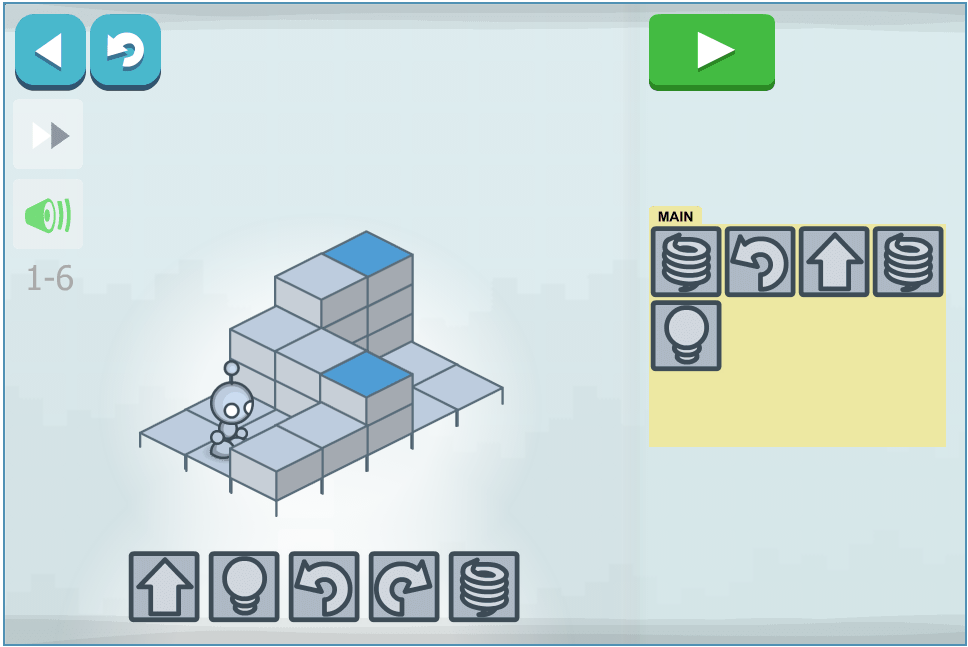
\includegraphics[width=0.8\textwidth]{lightbot1}
\end{figure}

Når du er fornøyd med programmet du har laget til roboten trykker du på den grønne pilen på toppen av skjermen, da kjøres programmet. At programmet ditt kjøres, betyr at alle kommandoene du har lagt inn utføres i rekkefølge. Du kan nå følge med på hva roboten gjør, for å se om programmet ditt gjør som du ville. Enten greier roboten å lyse opp alle de blå feltene, isåfall har du greid brettet. Eller så mislykkes roboten, det gjør ingenting, da trykker du bare på den oransje knappen for å resette roboten, og du kan så gjøre endringer til programmet før du prøver å kjøre det igjen.

\clearpage

Etter du har spillt igjennom de fire, fem første brettene, begynner du nok å få teken på hvordan du skal programmere roboten til å gjøre det du vil. Det du gjør når du spiller dette spillet, er faktisk programmering. For å være mer nøyaktig, så er spillet et eksempelt på noe vi kaller \emph{symbolsk programmering}, fordi du bruker symboler, eller ikoner, for å lage programmet ditt, istedenfor kode. Men ellers så er dette akkurat det samme som vi kommer til å gjøre når du skal lære å skrive Python.

For hvert brett så har du en konkret oppgave du har lyst til å løse, du har lyst til å lyse opp alle de blå feltene på brettet. For å klare det er det en del hindre du må komme deg forbi. Du starter å løse hvert brett ved å finne ut hvilke kommandoer du må bruke for å komme deg forbi hindrene og lyse opp feltene. Etter du har skjønnt hvordan du skal løse brettet, så `koder' du opp programmet ditt ved å velge de riktige instruksene. Når du har gjort dette, så tester du koden din ved å kjøre programmet. Hvis det er feil i koden, så retter du dem opp. Slik fortsetter du, helt til du har et helt program som løser hele brettet. Vi har nå oppsummert hva det vil si å programmere.

\subsection*{Oppsummering av programmeringstankegangen}

For å oppsummere programmeringstankegangen, så har jeg laget en liten figur. Ta en titt på den og se om du greier å knytte opp spillet Lightbot til de forskjellige stegene.

\vspace{1cm}

\begin{figure}[!h]
\centering
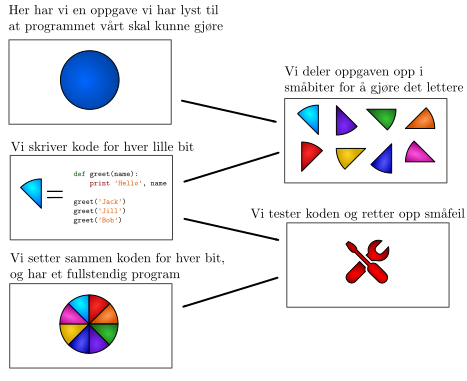
\includegraphics{programmering}
\end{figure}

\clearpage

\section*{Pythonprogrammering}

Nå som vi har fått inn grunntanken med programmering, la oss begynne å se på Python. Når dere skal programmere i Python så trenger dere en data hvor python er installert. Akkurat nå tar vi oss ikke tid til å installere det vi trenger, så vi velger å bruke en løsning på internet. Hvis vi går inn på nettsiden

\url{repl.it}

så kan du velge mellom mange forskjellige programmeringsspråk. Klikk på Python, og vi kommer inn i noe vi kaller en Python interpreter, der vi kan skrive og kjøre Python-kode. Nettsiden skal nå se ligne på dette
\begin{figure}[htpb]
	\centering
	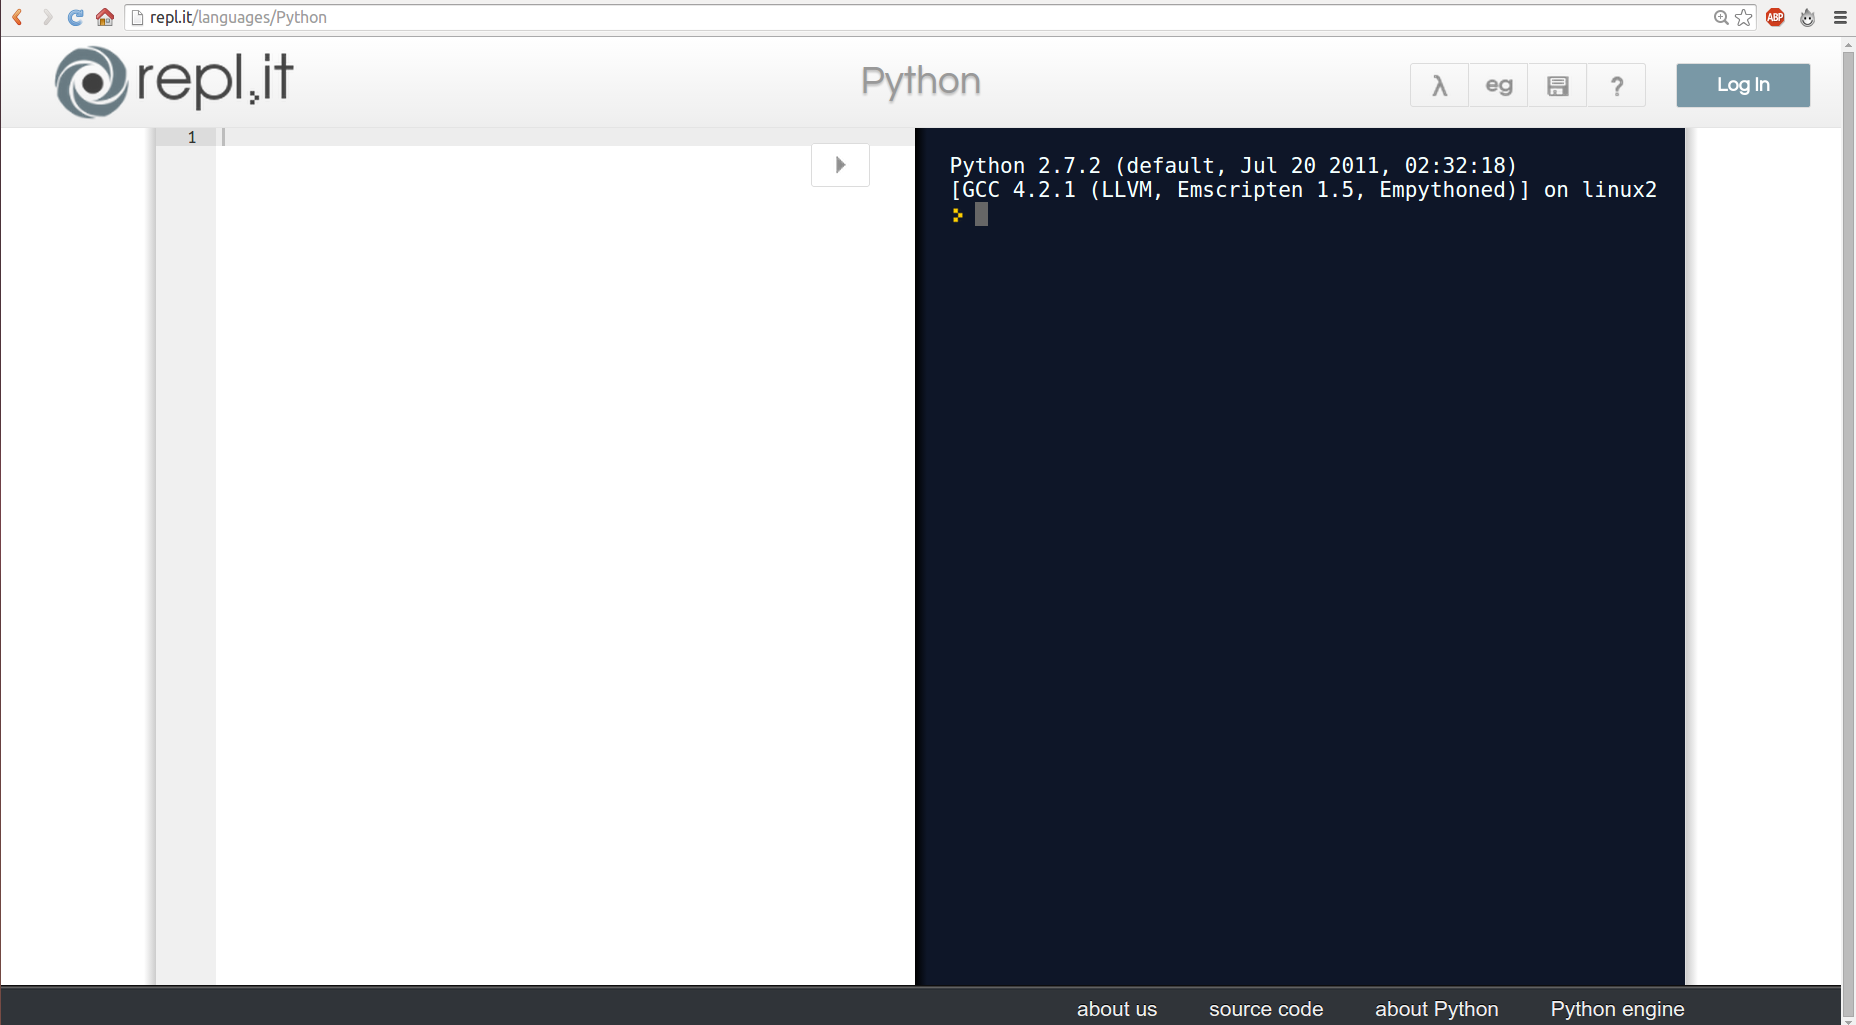
\includegraphics[width=\textwidth]{6hjBfs2}
\end{figure}

På venstre side av skjermen, i det hvite vinduet, er der vi skriver selve programmet vårt, vi kaller gjerne dette vinduet for editoren. I editoren skriver du koden din. På høyre side av skjermen, i det mørke-blå vinduet, er det resultatet av kjøringen din kommer. Vi kaller det blå vinduet for terminalen. Når du vil kjøre programmet du har skrevet i det hvite vinduet, så kan du trykke på pilen du ser øverst til høyre i det hvite vinduet (ca midt på skjermen), da kjøres programmet ditt. Når programmet kjøres, så utfører Python koden du har skrevet, linje for linje, fra toppen ned. Resultater fra kjøringen skrives ut i terminalen.

\subsection*{Ditt første Pythonprogram}

Nå er det på tide at du skal skrive ditt første Pythonprogram. Vi lar det være et utrolig enkelt program, kun bestående av linjen 
\begin{lstlisting}
print 'Hello, world!'
\end{lstlisting}
Skriv inn koden i editoren (det hvite vinduet), og trykk på pilen for å kjøre programmet ditt. Hva er det som skjer? Forhåpentligvis så vises skriften \emph{Hello, world!} i terminalen (det blå vinduet). La oss ta en titt på hva som har skjedd. Kodelinjen du har skrevet er en \verb+print+-kommando. I Python så er \verb+print+ et nøkkelord som betyr at noe skal vises (skrives ut) til terminalen. Det koden vår gjør er altså å bruke \verb+print+-kommandoen til å skrive ut en beskjed til terminalen.

Merk at i koden så har vi omringet beskjeden vi har lyst til å skrive ut med fnutter, \verb+''+, dette er fordi Python skal kunne skille mellom teksten i beskjeden og resten av koden. Vi kaller teksten i fnutter for en tekststreng, og tekststrenger tolkes aldri av Python som kode, den behandles bare som en tekst. Hvis du ser på terminalen, så ser du at Python ikke har inkludert fnuttene i det den har skrevet ut, det er det som er mellom fnuttene som er viktig. Merk at hele tekststrenger har blitt farget en egen farge i editoren, sånn at det er lett å skille mellom teksten som er kode, og teksten som ikke er kode. Så lenge vi skriver beskjeden vi vil skrive ut som en tekststreng, det vil si mellom de to fnuttene, så kan vi skrive hvilken som helst tekst vi ønsker. Prøv selv å endre beskjeden et par ganger og se at alt fungerer som det skal.

La oss nå prøve å ha to printkommandoer etter hverandre
\begin{lstlisting}
print "Hva skjera Baghera?"
print "Ingenting tingeling!"
\end{lstlisting}
Hva skjer når du kjører programmet nå? Hver av linjene i programmet er en \verb+print+-kommando som skriver ut en tekststreng. Python tolker koden linje for linje nedover, så den vil først behandle den ene print-kommandoen, og så den andre. Utskriftene til Terminalen havner etter hverandre, på hver sin linje. 

\section*{Variable}

Når vi skriver et dataprogram, så er det viktig at datamaskinen skal kunne huske på ting den trenger å vite. Vi får datamaskinen til å huske på ting ved å definere noe vi kaller variabler. Vi kan tenke på en variabel som en boks. La meg vise deg et eksempel, her er to linjer kode
\begin{lstlisting}
name = "Jonas"
alder = 23
\end{lstlisting}
Hva er det denne koden gjør? Den første kodelinjen sier \verb+name = Jonas+. Det jeg gjør med denne kommandoen er å fortelle Python navnet mitt. Mer teknisk kan jeg si at jeg lager en variabel som heter \verb+name+, og den inneholder navnet mitt, som er teksten `Jonas'. Det Python gjør når den behandler denne kodelinjen, er at den oppretter en variabel, tenk på det som en tom boks, som heter \verb+name+. Så putten den teksten `Jonas' inn i den boksen, så setter den boksen i arkivet. Tilsvarende sier den neste kodelinjen at det skal være en variabel som heter \verb+age+, og der ligger tallet 23.

Prøv å skriv et lignende program for deg selv, med ditt navn og din alder. Kjør programmet, hva skjer? Ingenting skjer, ihvertfall ikke som du kan se. Terminalen er helt tom. Python oppretter variablene, akkurat slik vi spør om, men den viser ikke i terminalen at den har gjort noe. For å få noe til å skje, så kan vi legge til en \verb+print+-kommando i bunn av programmet vårt
\begin{lstlisting}
print name
\end{lstlisting}
Hvis du kjører programmet nå, så ser du at navnet ditt skrives ut i terminalen. Det er fordi du ber Python skrive ut \verb+name+, det som skjer da er at Python sjekker om den har en variabel (en boks) som heter name, når den finner den riktige variabelen i minnet sitt (den riktige boksen fra arkivet), så sjekker den hva innholdet er, og skriver ut innholdet til terminalen. På samme måte kan vi skrive ut variabelen \verb+age+ til terminalen med kommandoen
\begin{lstlisting}
print age
\end{lstlisting}
Det du kan prøve på nå, er å skrive 
\begin{lstlisting}
print 'name'
\end{lstlisting}
eller 
\begin{lstlisting}
print 'age'
\end{lstlisting}
Hvis du gjør det, så ser du at du \emph{ikke} får skrevet ut navnet eller alderen din til terminalen. Det er fordi Python tolker det du prøver å skrive ut som tekststrenger, fordi du har skrevet dem med fnutter på sidene.

Merk at hvis du prøver å opprette to variabler med samme name, så overskrives rett og slett den originale variabelen. Prøv for eksempel programmet
\begin{lstlisting}
name = "Marius"
name = "Lise"

print name
\end{lstlisting}
Hva forventer du at skjer? Prøv selv!

\subsection*{Typer}

Du har nå sett at vi kan lage variable. Variabler har altså navn og innhold, men de har også en \emph{type}. Hvis vi ser på de to variablene vi nettopp lagde, så har vi \verb+name+, som inneholder en tekststreng, og \verb+alder+ som inneholder et tall. Når Python oppretter en variabel, så husker den ikke bare på navnet og innholdet, men den merker seg også hva slags innhold variabelen har.

Vi kan bruke kommandoen \verb+type+ til å sjekke hva slags type en variabel har. Her er et eksempelprogram
\begin{lstlisting}
location = "Oslo"
year = 2015
day = "4. januar"
temperature = -7.3

print type(location)
print type(year)
print type(day)
print type(temperature)
\end{lstlisting}
I dette programmet oppretter jeg først fire variable, så skriver jeg ut til terminalen hvilken type de har. Merk at kommandoen \verb+type+ sjekker typen til det du skriver inne i parantesen, sånn at \verb+type(sted)+ betyr typen til variabelen \verb+navn+. Når du kjører programmet får du denne utskriften i terminalen
\begin{lstlisting}
<type 'str'>
<type 'int'>
<type 'str'>
<type 'float'>
\end{lstlisting}
Vi ser altså at variabelen \verb+location+ har type `str', dette er en forkortelse for `string', og betyr altså tekststreng. Dette stemmer jo godt, fordi variabelen \verb+location+ inneholder jo en tekststreng. Variabelen \verb+year+ har type `int' som er en forkortelse for `integer'. Integer er engelsk og betyr heltall. Vi ser at \verb+day+ også er en `str', altså tekstreng. Til sist har vi \verb+temperature+ som har typen `float', som betyr flyttall. Et flyttall er egentlig bare et annet navn på et desimaltall. Vi ser altså at Python skiller på heltall og desimaltall.

\section*{Lister}

Hitil har du sett at variable har et navn, et innhold og en type. La oss se på en ny type variabel: lister. La oss si at du ikke bare ønkser at programmet ditt skal huske på et navn, men en hel skoleklasse. Det er veldig slitsomt å måtte opprette en variabel for hver enkelt elev. Det vi kan gjøre, er å opprette en enkelt variabel, hvor vi lagrer alle elevene sammen, det kan du gjøre sånn her
\begin{lstlisting}
students = ["Jake", "John", "Mary", "Lucy", "Alexander"]
\end{lstlisting}
Vi ser at vi har brukt firkantparanteser: \verb+[+ og \verb+]+ for å definere en liste, og inne i listen har vi skrevet 5 navn, alle adskilt med komma. Merk også at vi definerer hvert navn som hver sin tekststreng. Når du har definert en liste på denne måten, så kan du skrive den ut med \verb+print+, og selvfølgelig sjekke typen
\begin{lstlisting}
print students
print type(students)
\end{lstlisting}
Når du gjør det, så får du følgende utskrift i terminalen
\begin{verbatim}
[' Jake ', ' John ', ' Mary ', ' Lucy ', ' Alexander ']
<type 'list'>
\end{verbatim}
En annen ting du kan gjøre med en liste, er å sjekke hvor mange ting den inneholder, det gjør vi med \verb+len+, som forteller deg lengden på en liste
\begin{lstlisting}
print len(students)
\end{lstlisting}
forteller oss at det er 5 navn i lista.

En liste trenger ikke nødvendigvis inneholde tekststrenger, vi kan plassere hva som helst i dem. Vi kan for eksempel ha en liste med tall
\begin{lstlisting}
prices = ["299", "199", "4000", "20"]
\end{lstlisting}
Eller en blanding av tall og tekst
\begin{lstlisting}
my_list = ["Some text", 2, 2.3, 9, "Some more text"]
\end{lstlisting}
Du kan tilogmed legge lister inne i andre lister
\begin{lstlisting}
lists_in_lists = [[0, 2, 3], ["Mary", "Lucy", "Jake"]]
\end{lstlisting}
Siden en liste kan bestå av så og si hva som helst, så pleier vi å kalle det den inneholder for elementer. En liste er en rekke elementer.

Når vi først har definert en liste, for eksempel en liste over alle elevene i en skoleklasse
\begin{lstlisting}
students = ["Jake", "John", "Mary", "Lucy", "Alexander"]
\end{lstlisting}
Så kan vi gå inn i lista og hente ut ett bestemt navn. Det gjør vi med noe som heter indeksering, jeg kan for eksempel skrive
\begin{lstlisting}
print students[0]
print students[3]
\end{lstlisting}
Her så betyr \verb+students[0]+ det første elementet i lista, som altså er `Jake', mens \verb+students[3]+ betyr det fjerde navnet i lista, som er `Lucy'. Tallet vi skriver teller altså elementer utover i lista, og vi begynner å telle på 0. Det er kanskje litt rart, men sånn fungerer det altså.

Vi kan også overskrive et bestemt element i en liste. Si for eksempel at vi har funnet ut at vi har gjort en feil, Alexander i lista over heter egentlig bare Alex! Vel, da kan vi gå inn og endre bare den delen av lista. `Alexander' står på den 5 plassen i lista, så det er \verb+students[4]+ vi må endre, så da skriver vi
\begin{lstlisting}
students[4] = "Alex"
\end{lstlisting}
Hvis vi nå skriver ut hele lista på nytt med \verb+print students+ får vi utskriften
\begin{verbatim}
[' Jake ', ' John ', ' Mary ', ' Lucy ', ' Alex ']
\end{verbatim}
Så du ser at det er bare `Alexander' som har endret seg i lista.

Du kan også legge til ekstra elementer i listen din. Si for eksempel at du har glemt en av elevene i klassen din, da kan den personen legges til som følger
\begin{lstlisting}
students.append("Roger")
\end{lstlisting}
Hvis vi nå skriver ut lista får vi
\begin{verbatim}
[' Jake ', ' John ', ' Mary ', ' Lucy ', ' Alex ', 'Roger']
\end{verbatim}
Merk at elementer vi legger til med \verb+.append+ havner på enden av lista.

Siden vi kan legge elementer til en allerede eksisterende liste, så kan det av og til gi mening å lage en helt tom liste. Se for eksempel på denne koden
\begin{lstlisting}
my_list = []
my_list.append(1)
my_list.append(2)
my_list.append(3)
\end{lstlisting}
Her lager jeg først en helt tom liste, så begynner jeg å fylle den med tall etterpå.



\section*{Feilmeldinger}

Nå som du har begynnt å skrive din første Pythonkode kan det jo være at det har oppstått noen feil, og hvis du har gjort alt rett så langt, så dukker det opp noen feil snart. La oss ta en titt på feilmeldingene vi får når vi gjør feil i Python, og prøve å tolke dem litt. Når du programmerer kommer du til å gjøre mange feil og det er viktig å prøve å forstå hvorfor det gikk galt, det å tolke sine egne feilmeldinger er nok den aller beste måten å bli god til å programmere.

La oss skrive en \verb+print+-kommando feil med vilje
\begin{lstlisting}
prnt "Hello, World!"
\end{lstlisting}
Når du prøver å kjøre programmet nå, så får du en feilmelding ut. Den ser ut noe som dette:
\begin{verbatim}
File "<stdin>", line 1
    prnt "Hello, World!"
                       ^
SyntaxError: invalid syntax
\end{verbatim}

Det er alltid den nederste linjen i en feilmelding som er den viktigste, og der står det \verb+SyntaxError: invalid syntax+. Feilen vi har gjort er altså en \emph{syntaks}-feil. En syntaks-feil betyr at Python ikke skjønner det vi har skrever, vi har skrevet noe som rett og slett ikke gir mening. Når du får en syntaks-feil bør du altså sjekke at du har skrevet alt riktig, sånn som her ser vi at \verb+print+-kommandoen er skrevet feil. 

På linjene over prøver Python å informere oss hvor feilen er. Det står `line 1' på toppen, akkurat nå er det jo åpenbart at feilen må være i kodelinje 1, for det er alt vi har skrevet! Men i et program på flere hundre kodelinjer er det veldig nyttig å få vite hvilken linje feilen er på. 

La oss prøve en annen feil
\begin{lstlisting}
location = "Oslo"
print place
\end{lstlisting}
Hvis du kjører dette programmet får du feilmeldingen
\begin{verbatim}
Traceback (most recent call last):
File "<stdin>", line 2, in <module>
NameError: name 'place' is not defined
\end{verbatim}
Nå har du ikke lenger en syntaks-feil, fordi Python skjønner godt hva du har lyst til å gjøre her, det du har skrevet er helt riktig Python-kode. Problemet er derimot en \verb+NameError+, det er ganske enkelt fordi programmet først oppretter variabelen `location', og prøver deretter å printe ut variabelen `place'. Men det finnes ingen variabel med navn `place', så derfor får du en navn-feil---programmet prøver å bruke en variabel som ikke finnes.

La oss se på en siste feil
\begin{lstlisting}
students = ["John", "Jake", "Mary", "Marcus"]
print students[4]
\end{lstlisting}
Når programmet kjøres får du feilmeldingen
\begin{verbatim}
File "<stdin>", line 2, in <module>
    print students[4]
IndexError: list index out of range
\end{verbatim}
Vi ser at vi får en \verb+IndexError+ og det står `list index out of range'. Målet med \verb+print+ kommandoen er å skrive ut det fjerde navnet i lista, Marcus. Problemet er derimot at vi har glemt at Python starter å telle på 0, så Marcus har indeks 3! Dermed prøver vi å lese en del av lista som ikke finnes, og vi får en `index out of range'-feil.

\section*{Mer om printing}

Så langt har du sett at du kan skrive ut både tekststrenger og variable, la oss nå kombinere dem. Ta en titt på følgende program
\begin{lstlisting}
name = "Silje"
print "Hei", name, "! Hvordan har du det idag?"
\end{lstlisting}
Her bruker vi \verb+print+-kommandoen til å skrive ut 3 ting etterhverandre. Hvis du kjører programmet så ser du at de tre tingene vi skriver ut havner på samme linje, ikke hver sin linje, det er fordi de alle hører til samme \verb+print+-kommando.

Hvis du ser nærmere på utskriften, så kan du legge merke til at Python har lagt inn et mellomrom mellom hver av tingene vi skriver ut, så i terminalen står det 
``Hei Silje ! Hvordan har du det idag?''. Det er jo litt dumt at det er et ekstra mellomrom mellom `Silje' og `!', så la oss se på en annen måte vi kan skrive ut en beskjed og en variabel samtidig.
\begin{lstlisting}
name = "Silje"
print "Hei %s! Hvordan har du det idag?" % name
\end{lstlisting}
Prøv å kjør dette programmet? Nå ble beskjeden akkurat slik vi ønsket. Men hva er det vi egentlig har gjort her? Vi ser at vi prøver å skrive ut en tekststreng, men inne i tekstrengen står det \verb+%s+. Når vi skriver \verb+%s+ inne i en tekststreng, så lager vi et slags hull i strengen, der vi kan fylle inn en variabel. Vi skriver \verb+% name+ bak tekstrengen, fordi det er denne variabelen vi ønsker å fylle inn i hullet. Grunnen til at vi skriver \verb+%s+ i strengen er fordi \verb+s+ står for streng, siden vi fyller inn med en variabel som er en tekststreng.

Vi kan lage så mange hull i en tekst som vi ønsker, her er et eksempel
\begin{lstlisting}
name = "Silje"
age = 18
location = "Drammen"

print "Jeg heter %s, er %i og kommer fra %s." % (name, age, location)
\end{lstlisting}
Nå ser vi at det er 3 hull i teksten, det er to strenger merket med \verb+%s+ og et heltall merket med \verb+%i+ (husk at integer betyr heltall på engelsk). Bak strengen har vi listet opp tre variable som skal fylles inn i teksten. Merk at vi har satt parantes rundt dem, og at de kommer i samme rekkefølge som hullene i teksten.

\subsection*{Dataprogrammer som snakker med brukeren}

Så lang har vi bare laget programmer som gjør noe enkelt og slutter helt av seg selv. Men de fleste programmer dere bruker i hverdagen er jo laget for å ha en interaksjon med brukeren. La oss derfor stille brukeren av programmet noen spørsmål, det kan vi gjøre med kommandoen \verb+raw_input+. Her er et eksempel
\begin{lstlisting}
weather = raw_input('Hi! How is the weather today?')
print "The weather seems to be %s today!" % weather
\end{lstlisting}
Når Python utfører denne kodelinja, så skrives spørsmålet i parantesen ut i terminalen, og så venter den på at brukeren som har kjørt programmet skal skrive inn et svar. Prøv å kjør programmet, skriv inn et svar på spørsmålet og trykk enter for å fortsette videre i programmet. Det du (brukeren) svarer på spørsmålet blir så lagret i variablen \verb+weather+. Etter du har trykket enter, fortsetter programmet. I vårt tilfelle går den da videre til å skrive ut en beskjed, hvor svaret brukeren ga brukes.

\subsection*{Oppsummering uke 1}

\begin{itemize}
	\item Å programmere betyr å lage et dataprogram. Dette gjør vi ved å skrive kode i et bestemt programmeringsspråk. Før vi kan gå igang med å kode må vi ofte bryte ned oppgaven vi skal løse i små biter.
	\item Datamaskinen husker ting i form av \emph{variabler}, vi kan opprette variabler ved å gi dem navn og et innhold. Python gir også variabelen en type, som vi kan sjekke ved å bruke kommandoen \verb+type()+.
	\item Vi kan lage lister ved hjelp av firkantparanteser: \verb+[+, \verb+]+. Lister er variabler som inneholder flere ting, de kan inneholde så mange elementer vi vil, av alle slag.
	\item Når vi har laget en liste, så kan vi finne lengden på lista ved å bruke \verb+len()+, vi kan også legge til fler elementer med \verb+my_list.append()+, og vi kan gå inn og lese ut eller enkelte elementer ved indeksering: \verb+my_list[2]+. Husk at indekseringen begynner på 0. Så første element er \verb+my_list[0]+, andre element er \verb+my_list[1]+ og så videre.
	\item For å skrive ut noe til terminalen kan vi bruke \verb+print+-kommandoen, vi kan skrive ut både variabler og tekststrenger.
	\item Vi kan skrive ut flere ting etterhverandre hvis vi skiller dem med komma: \verb+print ting1, ting2+, eller vi kan skrive ut tekster som vi fyller inn med variabler: \verb+print "Hei, jeg heter %s" % name+.
	\item Vi kan spørre brukeren et spørsmål med kommandoen \verb+raw_input()+, i parantesen skriver du spørsmålet som en tekststreng.
	\item Det er lett å gjøre feil i programmering, men det gjør ingenting. Når vi kjører et program med feil i, får vi en feilmelding som prøver å fortelle oss hva som har gått galt.
\end{itemize}

\clearpage

\section*{Oppgaver til uke 1}

\subsection*{Oppgave 1 --- Printing}
\begin{itemize}
	\item[(a)] Lag et program som skriver ut teksten ``Hello, World!'' til skjermen.
	\item[(b)] Lag et program hvor du lagrer navnet ditt som en variabel, og deretter skriver ut lengden på navnet ditt med kommandoen \verb+len(name)+.
	\item[(c)] Lag et program som spør brukeren om navnet dems, og deretter skriv en beskjed tilbake som bruker navnet de har gitt. \\
	\textbf{Hint:} Du kan spørre brukeren et spørsmål med \verb+raw_input+-kommandoen. 
\end{itemize}

\subsection*{Oppgave 2 --- Lister}
Ta en titt på følgende program
\begin{lstlisting}
x = [1]
x.append(2)
x.append(3)
print x 
x[0] = 4
print x
print len(x)
print type(x)
print type(x[0])
\end{lstlisting}
\begin{itemize}
	\item[(a)] Uten å faktisk kjøre programmet, hva tror du at utskriften fra denne koden kommer til å være?
	\item[(b)] Kjør koden for å se om du hadde rett.
\end{itemize}



\subsection*{Oppgave 3 --- Adjektivhistorie}
\begin{itemize}
\item[(a)] Spør brukeren om 5 adjektiv og lagre dem i 5 forskjellige variable. \\
	\textbf{Hint:} Adjektiv er beskrivende ord som for eksempel `liten' og `stor'.
\item[(b)] Test programmet ditt ved å skrive ut alle 5 adjektivene i terminalen.
\item[(c)] Skriv en adjektivhistorie og print den slik at de 5 adjektivene brukeren har gitt fylles inn i historien.
\item[(d)] Test programmet ditt.
\item[(e)] Hvis alt funker som det skal kan du nå gjemme editoren din, kjør programmet og få en venn til å fylle ut adjektivene.
\end{itemize}

\subsection*{Oppgave 4 --- Lightbot}
\begin{itemize}
\item[(a)] Spill igjennom alle brettene.
\item[(b)] \textbf{Utfordring}: Klarer du å løse brett 2--1 med bare 7 kommandoer? Hva med brett 2--2?
\item[(c)] \textbf{Utfordring}: Hvor få kommandoer klarer du å bruke for å løse 2-6? Det beste jeg har fått til er 15 kommandoer!
\end{itemize}

\clearpage

\section*{Matematikk i Python}

Programmering og matematikk er tett knyttet sammen, 


Du kan bruke vanlige matematiske operasjoner som \verb!+! og \verb!-! i Python, for å gjøre utregninger. Vi kan for eksempel skrive
\begin{lstlisting}
print 12 + 49
print 24.4 - 6.3
\end{lstlisting}
Husk at vi fortsatt må bruke \verb+print+-kommandoen for å faktisk skrive ut resultatet til terminalen. Hvis du bare skriver \verb!2+2! på en kodelinje, så vil Python regne ut svaret, men så vil den ikke bruke det svaret til noe så utregningen er ganske bortkastet.

Du kan også lagre resultatet fra en utregning i en variabel
\begin{lstlisting}
addition = 72 + 23
subtraction = 108 - 204
multiplication = 108 * 0.5
division = 108/9
\end{lstlisting}
I hvert tilfelle her så regner Python først ut det som er til høyre for likhetstegne, og lagrer resultatet i variabelen som står til ventre for likhetstegnet. Merk også at \verb+*+ er multiplikasjon og \verb+/+ divisjon. Et problem med divisjon i Python er at det finnes noe som heter heltallsdivisjon. Når du gjør beregningen \verb+108/9+, så ser Python at du prøver å dele et heltall på et heltall (husk at Python skiller på heltall og desmialtall), siden du deler heltall på hverandre tror Python at du vil ha et heltall som resultat! Prøv for eksempel å skrive
\begin{lstlisting}
print 5/2
\end{lstlisting}
Svaret du får er 2, ikke 2.5. Det er fordi vi har heltalldivisjon, og heltalldivisjon forteller deg bare hvor mange ganger telleren (her 5) går opp i nevneren (2), siden 5 går opp i 2 to ganger, får vi svaret 2. Hvordan unngår du heltallsdivisjon? Hvis et av tallene som inngår i divisjonen er et flyttall, så vil Python skjønne at du har lyst på flyttallsdivisjon (det du kjenner som `vanlig' divisjon). Vi har altså et par muligheter for å få til dette
\begin{lstlisting}
print 5.0/2.0
print 5.0/2
print 5/2.0
print 5./2
print float(5)/2
\end{lstlisting}
Alle disse måtene å dele tallene på hverandre vil gi svaret 2.5. Alle måtene fungerer fordi minst ett av tallene som inngår i divisjonen er flyttall, i det første tilfellet skriver vi \verb+5.0+ og \verb+2.0+ istedenfor \verb+5+ og \verb+2+, men vi ser at det også går å bare skrive for eksempel \verb+5.+. I det siste tilfellet så endrer vi typen til tallet \verb+5+ direkte med kommandoen \verb+float+. 

Du kan kombinere så mange matematiske operasjoner som du vil
\begin{lstlisting}
print 305/2.0 + 222*5 - 3
\end{lstlisting}
Python utfører operasjonene i riktig matematisk rekkefølge, multiplikasjon og divisjon før addisjon og subtraksjon osv. Hvis du for eksempel skriver 
\verb!1+2*3! så blir resultatet 7, \emph{ikke} 9. Hvis du vil at utregningen skal skje i motsatt rekkefølge kan du bruke paranteser akkurat sånn som man gjør for hånd: \verb!(1+2)*3! gir resultatet 9.

Du kan også regne med variabler, så du kan for eksempel skrive
\begin{lstlisting}
a = 3.0
b = 4.0
print 4*a
print a + b 
print a * (b+2)
\end{lstlisting}

En ting det er verdt å være obs på, er at likhetstegnet i Python: \verb+=+, ikke er det samme som i matte. Hvis du for eksempel skriver
\begin{lstlisting}
x = 1
x = x + 2
\end{lstlisting}
Så er dette helt riktig Python kode som gir mening. I matematikk derimot, så gir ikke ligningen
$$x = x + 2,$$
noe mening i det hele tatt. Hvordan kan noe være lik seg selv \emph{pluss to}?

Du må huske at likhetstegnet i Python kun brukes for å definere variable. La oss se på hvordan Python tolker kodelinjen
\begin{lstlisting}
x = x + 2
\end{lstlisting}
Først ser den på høyre side av likhetstegnet og regner ut det som står der. Vi har definert variabelen \verb+x+ til å være 1, så på høyre side står det \verb!1+2! som gir resultatet 3. Deretter ser den på venstre side av likehetstegnet, der skal den lagre resultatet. Siden \verb+x+ allerede er definert i programmet, så blir den rett og slett overskrevet av den nye kommandoen. Etter programmet har kjørt, så finnes det altså 1 variabel, \verb+x+ som har verdien 3. Du kan sjekke det selv ved å skrive ut resultatet med \verb+print x+.

Hvis du syns likhetstegnet er litt vansklig å forstå, så kan det kanskje hjelpe å tolke det som en slags pil istedet, som egentlig gir mer mening
\begin{lstlisting}
x <- 1
x <- x + 2
\end{lstlisting}
Dette er \emph{ikke} gyldig kode, det er bare for å forklare hvordan ting fungerer i bakgrunnen.

\subsection*{Eksempel: Restaurantregning}
La oss nå se på et eksempel hvor vi regner litt. La oss si vi er på restaurant, vi har spist og drukket for et grunnbeløp, men i tilegg til det kommer merverdiavgift (mva) og tips. La oss lage et program hvor vi først definerer grunnbeløpet, hvor mye mva vi må betale, og hvor mye tips vi har lyst til å gi. Deretter regner vi ut totalen vi må ut med og skriver den til terminalen. 

Først definerer vi grunnbeløpet, mva, og tips. 
\begin{lstlisting}
basispris = 240
mva = 0.25
tips = 0.1
\end{lstlisting}
Her sier vi at vi grunnbeløpet er 240 kr, vi må betale 25 \% mva, som er standarden i Norge, og vi har lyst til å tipse 10 \%. Merk at jeg har skrevet prosentene som desimaltall ved å dele på 100, det er så det skal være lettere å regne med.

Nå skal vi regne ut totalen, først legger vi inn mvaen, deretter tipsen
\begin{lstlisting}
pris = basispris + basispris*mva
tips = pris * tips
total = pris + tips
\end{lstlisting}

Til slutt kan vi skrive ut resultatet med en liten beskjed
\begin{lstlisting}
print "Totalprisen ble %.2f kr, hvorav %.2f er tips." % (total, tips)
\end{lstlisting}
Når jeg skriver ut bruker jeg \verb+%.2f+, \verb+f+ fordi det er flyttall jeg skriver ut, \verb+.2+ betyr at jeg bare vil ha med to desimaler i svaret som skrives ut. Prøv selv med bare \verb+%f+ og se hva som skjer, du får fryktlig mange desimaler.

\section*{Mer avansert matematikk}

Du kan regne med potenser ved å bruke to produkttegn på rad \verb+**+. For eksempel vil
\begin{lstlisting}
print 4**2
print 2**3
\end{lstlisting}
gi resultatetene 16 og 8 fordi $4^2=16$ og $2^3 = 8$.

Hvis vi har lyst til å ta kvadratroten av et tall, for eksempel $\sqrt{49}$, så finnes det en kommando som gjør dette, men den må vi først \emph{importere}. Grunnleggende Python er et ganske lite og enkelt programmeringsspråk, men det finnes tusenvis av pakker man kan inkludere for å gjøre det mer komplekst og kraftig. Nå skal vi drive med matte, og importerer derfor en kommando fra biblioteket som heter `math', det gjør vi som følger
\begin{lstlisting}
from math import sqrt
\end{lstlisting}
Vi har nå importert \verb+sqrt+ (står for square root, eller kvadratrot på norsk) fra `math'. Vi kan nå bruke \verb+sqrt+ som alle andre kommandoer i Python, for eksempel til å regne ut $\sqrt{49}$:
\begin{lstlisting}
print sqrt(49)
\end{lstlisting}
Alle kan lage ekstrabiblioteker til Python og det finnes derfor mange tusen biblioteker vi kan laste ned og bruke fritt når vi koder. Det finnes pakker for å lage grafikk, musikk, jobbe med nettsider osv. Hvis vi for eksempel ønsker å bruke Python til å lage et spill eller en iPhone app, så finnes det altså pakker til Python som gjør den jobben mye lettere for oss.

Nå tilbake til pakken `math'. Vi importerte kvadratrotfunksjonen derfra. En annen ting vi kan importere er tallet $\pi$. Prøv å skrive
\begin{lstlisting}
from math import pi 
print pi
\end{lstlisting}
Nå har vi ikke importert en ny kommando fra math, men istedet en variabel, som inneholder tallet $\pi$ til mange, mange desimaler.

I math finnes det mange andre funksjoner og konstanter vi kan importere, men det er nok ikke så mange du har bruk for akkurat nå. Etterhvert som du lærer mer matematikk i for eksempel 1T matte, så kommer du til å lære om matematiske funksjoner som eksponentialfunksjonen, sinus, cosinus, tangens og fakultet. Mattebibloteket inneholder alle disse funksjonene og er derfor veldig nyttig når man skal drive med matte.

\section*{Funksjoner}

Vi skal nå begynne å snakke om funksjoner. Funksjoner er noe av det mest fundamentale og viktige i programmering. Funksjoner lar oss definere egne kommandoer, og på den måten kan vi effektivisere koden vår enormt mye.

Du har allerede sett eksempler på funksjoner når du spilte Lightbot, der ble de kalt procedures. Når vi har en del kode som gjentas i et program, så er det mer effektivt å definere dem som en funksjon. Når vi har definert en funksjon, så kan vi bruke den ved å \emph{kalle på den}. 

I bildet under, så er det akkurat det vi gjør. I tillegg til hovedprogrammet vårt, så har vi et eget vindu hvor vi definerer funksjonen \verb+P1+, i hovedprogrammet så kan vi da kalle på \verb+P1+, da utføres alle kommandoene som ligger i definisjonen av funksjonen.

\begin{figure}[h!]
\centering
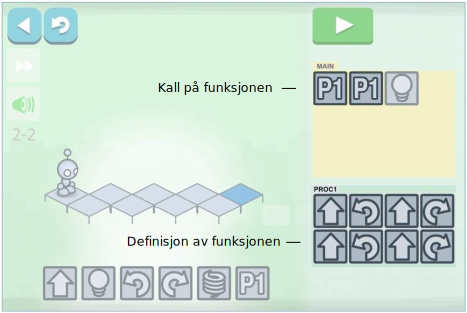
\includegraphics[width=\textwidth]{func2}
\end{figure}

I Python kan du definere funksjoner med nøkkelorder \verb+def+, en forkortelse for `define'. Vi gir funksjonen vårt et navn og skriver all koden som inngår i funksjonen med et innrykk, la oss se på et eksempel
\begin{lstlisting}
def greet():
	print "Hello, world!"

greet()
\end{lstlisting}
I denne koden ser du at kodeordet \verb+def+ brukes for å starte definisjonen av en funksjon, navnet jeg gir funksjonen min er \verb+greet+, parantesene må være der, og vi kommer tilbake til hvorfor. Etter den første linjen, så kommer selve koden i funksjon. All koden som inngår i funksjonen må få et innrykk, eller indentering. Du kan lage et slikt innrykk med tab-knappen (du finner den rett over Caps Lock knappen, på venstre side av tastaturet). I dette tilfellet er det bare en enkelt linje som har fått innrykk, sånn at funksjonen vår består bare av 1 kodelinje.

På bunn av koden så kaller vi på funksjonen ved å skrive navnet på funksjonen med paranteser. Når vi gjør det så kjører Python koden som er inne i funksjonen. Merk at vi kan kalle på funksjonen så mange ganger vi vil, hvis vi skriver
\begin{lstlisting}
greet()
greet()
greet()
\end{lstlisting}
så skrives ``Hello, World!'' ut tre ganger i terminalen.

Så langt er funksjoner i Python helt like de du så i Lightbot, men nå skal vi innføre en forskjell som gjør funksjoner i Python mye bedre, \emph{input}. Det er kanskje lettest å vise med et eksempel
\begin{lstlisting}
def greet(name):
	print "Hi there %s, nice to meet you!" % name

greet("John")
greet("Mary")
\end{lstlisting}
Funksjonen heter det samme som før, men nå står det ikke bare tomme paranteser, det står \verb+(name)+, dette betyr at funksjonen forventer at brukeren skal gi funksjonen noe input når man kaller på den. Slik input kalles for argumenter, vår funksjon forventer å få et navn som argument. Når du ser på koden inne i funksjonen skjønner du kanskje hvorfor, det funksjonen gjør er å skrive ut en beskjed som inneholder navnet man bruker til å kalle på funksjonen. Når du kaller på en funksjon som skal ha argumenter, så skriver du dem inn i parantesene når du kaller på funksjonen, slik som er vist i bunn av koden.

Funksjonene jeg har vist deg hitil, har alle skrevet noe ut til terminalen, men det vi vanligvis vil at en funksjon skal gjøre, er å \emph{returnere} noe. At en funksjon returnerer noe vil rett og slett si at den gir noe tilbake, vi kan tenke på det som funksjonens \emph{output}. Tenk en stund på kvadratrotfunksjonen vi importerte fra \verb+math+-biblioteket. Vi importerer \verb+sqrt+, og det er faktisk en funksjon! Tenk på når du bruker den, da må du enten skrive ut resultatet med \verb+print+:
\begin{lstlisting}
print sqrt(4)
\end{lstlisting}
eller du kan lagre resultatet i en variabel
\begin{lstlisting}
result = sqrt(4)
\end{lstlisting}
Ta en titt på det siste tilfellet, her definerer vi en variabel som heter \verb+result+. Som forklart tidligere, vil Python her først regne ut det som er på høyre side av likehetstegnet, og så lagre resultatet i variabelen på venstre side av likhetstegnet. Spørsmålet er da: hva er egentlig resultatet av et funksjonskall? La oss se på et eksempel hvor vi bruker \verb+return+ i funksjonen vår
\begin{lstlisting}
def double(x):
	return 2*x
\end{lstlisting}
Her definerer jeg en funksjon som heter \verb+double+, den tar et tall \verb+x+ inn, og \emph{returnerer} $2x$, altså det dobbelte. Jeg kan nå bruke \verb+double+ på alt av tall. Men her bør jeg passe meg litt. Hvis jeg bare skriver:
\begin{lstlisting}
double(2)
\end{lstlisting}
Så skjer det ingenting, det er fordi funksjonen selv ikke printer noe, jeg må istedet skrive 
\begin{lstlisting}
print double(2)
\end{lstlisting}
eller 
\begin{lstlisting}
result = double(2)
print result
\end{lstlisting}

Når Python ser kommandoen \verb+print double(2)+, så må den først finne ut hva den skal skrive ut til terminalen, så den kjører koden i \verb+double+-funksjonen, der ganges $2\cdot2$ og vi får resultatet 4. Så returneres resultatet, altså tallet $4$. Det at resultatet returneres betyr at Python skjønner at det er dette som skal skrives ut til terminalen.

Hvis vi istedet hadde laget double med en \verb+print+, istedet for en \verb+return+, sånn her:
\begin{lstlisting}
def double(x):
	print 2*x
\end{lstlisting}
Så kan vi skrive bare
\begin{lstlisting}
double(2)
\end{lstlisting}
For å få skrevet ut resultatet til terminalen. Men nå vil dette gi et rart resultat
\begin{lstlisting}
result = double(2)
print result
\end{lstlisting}
Hva er det egentlig som skjer her? Prøv å kjør programmet og se hva du får ut. Først får du skrevet ut tallet 4 til terminalen, dette skjer allerede i den første kodelinja når Python ser funksjonskallet til \verb+double+. Men så skal Python lagre resultatet i result, men siden vi ikke har noen \verb+return+-kommando i funksjonen vår, så vet ikke Python hva den skal lagre i \verb+result+, så derfor er \verb+result+ rett og slett en helt tom variabel. Når vi da på neste linje prøver å skrive ut \verb+result+, så står det bare \verb+None+.



For å oppsummere. I Python så har alle funksjoner et navn, de kan ta null, en eller fler inputs og gi null, en eller flere outputs. All kode som skal være en del av koden må få et innrykk og for å returnere noe fra funksjonen (output) bruker du \verb+return+-kommandoen. Her er malen for en funksjon
\begin{lstlisting}
def my_function(input1, input2)
	...
	...
	...
	return output1, output2
\end{lstlisting}

Før vi går videre anbefaler jeg deg å tenke litt på hvorfor vi egentlig kaller det å returnere. Vel, en ting er jo at funksjonen gir noe tilbake, et resultat av noe slag, det er jo greit nok. Men det er også en annen grunn. Husk at jeg har forklart at Python alltid tolker koden din linje for linje, en kommando av gangen. Når du kaller på en funksjon, så utfører Python den koden som er definer inne i den funksjonen, så på en måte kan du tenke på det som at Python gjør er hopp i koden din, den hopper inn i funksjonskoden. Når du gir en \verb+return+-kommando, så sier du at funksjonen er ferdig. Det betyr at Python kan gå tilbake til det der den var i den originale koden og fortsette å tolke neste linje med kode, altså at den kan returnere til der den var. Dette konseptet illustreres ganske godt i Lightbot, der hver kommando som utføres lyser opp i programmet ditt! Når du bruker en funksjon, så ser du at hver kommando i funksjonsboksen lyser opp og utføres før programmet `returnerer' til hovedprogrammet og fortsetter.


\subsection*{Funksjoner i matematikk}

Jeg har nå vist deg litt hvordan du kan lage funksjoner i Python. Funksjoner er en av de viktigste konseptene i programmering, og nesten uansett hva slags program du skriver eller hvilket språk du bruker, kommer du til å bruke mye funksjoner. Men funksjoner er ikke bare viktig i programmering, det er også viktig i matematikk.

I matematikken kan du tenke på en funksjon som en slags regel som gjør om et tall, til et annet tall. Eller du kan tenke på det som en slags maskin, du mater et tall, gjerne kalt $x$ inn en funksjon, ofte kalt $f$. Resultatet skriver vi $f(x)$, og du kan lese dette som `resultatet når funksjonen $f$ virker på tallet $x$'. Ofte så sier man bare `$f$ av $x$' for $f(x)$.

\begin{figure}[h]
\centering
	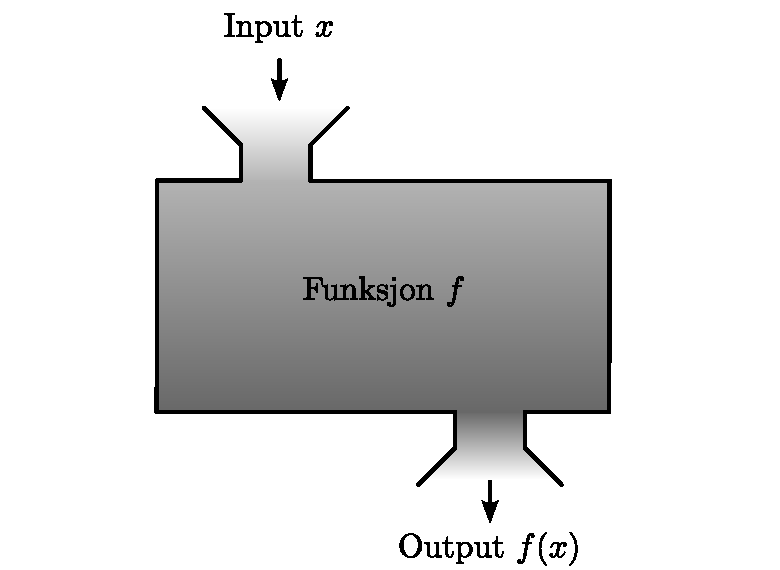
\includegraphics[width=0.6\textwidth]{function_blackbox}
\end{figure}

Et eksempel på en matematisk funksjon er for eksempel
$$f(x) = x^2 + 2x + 1,$$
Her definerer vi akkurat hva funksjonen vår gjør med et tall $x$. Vi kan nå sette inn for hva som helst av tall vi vil for $x$, her er et par eksempler
\begin{align*}
f(0) &= 0^2 + 2\cdot 0 + 1 = 1, \\
f(1) &= 1^2 + 2\cdot 1 + 1 = 4, \\
f(2) &= 2^2 + 2\cdot 2 + 1 = 9, \\
\end{align*}

Funksjoner er noe av det viktigste i matematikken, og det er på ungdomsskolen dere begynner å lære om dem. Når dere starter på videregående matematikk kommer det til å handle mye om funksjoner, og der lærer man om \emph{derivasjon} og \emph{integrasjon}, som handler mye om funksjoner. Hvis noen av dere en dag tar matematikk på et enda høyere nivå, kommer dere til å merke at det aller meste handler om funksjoner.

Jeg kommer ikke til å gå mer inn på matematiske funksjoner i dette kurset, siden vi fokuserer på programmering, og ikke nødvendigvis matematikk. Men matematiske funksjoner og funksjoner i programmering har veldig mye til felles, og det å ha forståelse for matematikk kommer til å hjelpe mye når man skal skrive kode og visa versa.


\section*{Oppsummering av uke 2}

\begin{itemize}
	\item Du kan bruke Python som en kalkulator med vanlige matematiske operasjoner: \verb!+!, \verb!-!, \verb!*! og  \verb!/!. Du kan ta potens med \verb!**!.
	\item Du må være forsiktig når du bruker divisjon for Python bruker \emph{heltalls\-divisjon}. For å unngå dette må du definere minst et av tallene som inngår i divisjonen som et desimaltall
	\item Python gjør kalkulasjoner i riktig matematisk rekkefølge. Du kan bruke paranteser for å bestemme rekkefølgen operasjonene gjøres i, akkurat som for hånd.
	\item Likhetstegn betyr \emph{ikke} det samme i programmering som det gjør i matematikk. I programmering betyr likhetstegn bare at du oppretter en variabel, i matematikk betyr det rett og slett at to ting er helt like. For eksempel \verb!x=x+2! fungerer fint i programmering, men ikke i matte.
	\item For mer avansert matematikk kan du importere ting fra et ekstrabibliotek. For eksempel kan du importere kvadratrot ved å skrive \begin{lstlisting}
from math import sqrt
	\end{lstlisting} På samme måte kan du importere konstanter som $\pi$.
	\item Vi kan definere funksjoner i Python som fungerer som egne kommandoer. De kan ta input, og kan returnere et output. Etter vi har definert en funksjon, så kan vi kalle på den så mange ganger vi vil. Koden for å skrive en funksjon er strukturert som følger
\begin{lstlisting}
def my_function(input1, input2)
	...
	...
	...
	return output1, output2
\end{lstlisting}

\end{itemize}

\clearpage

\section*{Oppgaver til uke 2}

\subsection*{Oppgave 1 --- Kalkulator}
Regn ut følgende ting og skriv resultatene til terminalen.
	\begin{itemize}
		\item[(a)] $4\cdot5+2$
		\item[(b)] $2^{10} $
		\item[(c)] $(-1)\cdot(-1)$
		\item[(d)] $\sqrt{36}$ \hspace{1cm} \textbf{Hint:} Du må importere \verb+sqrt+-funksjonen
		\item[(e)] $2 + 3\cdot(4-1+7)$
		\item[(f)] $\frac{1}{3} + \frac{2}{3}$
	\end{itemize}
Syns du resultatene ser rimelige ut?

\subsection*{Oppgave 2 --- Gjett på resultatet}
Ta en titt på følgende program
\begin{lstlisting}
y = 3
print y 
y = y + 4
print y 
y = y*y 
print y
\end{lstlisting}
\begin{itemize}
	\item[(a)] Uten å faktisk kjøre programmet, kan du si hva som vil vises i terminalen når programmet kjøres?
	\item[(b)] Etter du har prøvd å gjette på hva som vil vises i terminalen, kjør koden og se om du hadde rett.
\end{itemize}

\section*{Oppgave 3 --- Finn feil!}
Finn feilen i følgende program (det er en feil per program). Kjør gjerne programmet for å se feilmeldingen de produserer! Rett opp programmene så de fungerer som de skal.
\begin{itemize}
	\item[(a)] 
\begin{lstlisting}
name = Per 
print "Hi there %s!" % name
\end{lstlisting}

\item[(b)] 
\begin{lstlisting}
x = 24
y = 36
print X + y
\end{lstlisting}

\item[(c)] 
\begin{lstlisting}
def greet(name)
	print "Hi there %s" % name
\end{lstlisting}

\item[(d)] 
\begin{lstlisting}
location = "Oslo"
temperature = -18
print "The temperature in %s is now %s" % (location, temperature)
\end{lstlisting}

\item[(e)] 
\begin{lstlisting}
def double(x):
	result = 2*x

print double(2)
\end{lstlisting}
\end{itemize}

\subsection*{Oppgave 4 --- Kvadrattall}
Skriv en funksjon som tar et tall som input, og returnerer kvadrattallet. \\ \textbf{Hint:} Et kvadrattall er et tall ganget med seg selv, for eksmepel så er $3\cdot 3 = 9$, så 9 er kvadrattallet til 3.

\subsection*{Oppgave 5 --- Temperaturomregning}
For å regne oss om fra en temperatur oppgitt i grader Celsius $C$, til grader oppgitt i Fahrenheit $F$, bruker vi formelen
$$F = \frac{9}{5}C + 32.$$

\begin{itemize}
	\item[(a)] Lag en funksjon som tar en temperatur i celsius som input, og returnerer temperaturen i Fahrenheit. \\
	\textbf{Hint:} Funksjonen din bør se noe ut som dette (fyll inn for prikkene)
	\begin{lstlisting}
	def celsius_to_fahrenheit(C):
		...
		return F
	\end{lstlisting}
	\textbf{Hint:} Du kan kalle funksjonen din med for eksempel
	\begin{lstlisting}
	print celsius_to_fahrenheit(20)
	\end{lstlisting}
	\item[(b)] Sjekk at funksjonen din funker ved å vise at 
	\begin{itemize}
		\item[$\star$] 0$^\circ$ Celsius svarer til 32$^\circ$ Fahrenheit
		\item[$\star$] $-40^\circ$ Celsius svarer til $-40^\circ$ Fahrenheit
		\item[$\star$] $100^\circ$ Celsius svarer til $212^\circ$ Fahrenheit
	\end{itemize}
\end{itemize}


% \section*{Oppgave 1}
% \begin{itemize}
%     \item[(a)] Lag et skript som skriver ut teksten "Hello, World!" til skjermen.
%     \item[(b)] Lag et skript som skriver ut verdien av 4*5+2 til skjermen, blir resultatet annerledes om du skriver 2+4*5?
%     \item[(c)] Lag et skript som regner ut $2^{10}$ og skriver resultatet til skjermen.
%     \item[(d)] Lag et skript som regner ut $\sqrt{3}$ og skriver resultatet til skjermen. Her må du først importere \verb+sqrt+-kommandoen (squareroot) fra pylab.
% \end{itemize}

% \section*{Oppgave 2}
% For å regne oss om fra en temperatur oppgitt i grader Celsius $C$, til grader oppgitt i Fahrenheit $F$, bruker vi formelen
% $$F = \frac{9}{5}C + 32.$$
% \begin{itemize}
%     \item[(a)] Lag et skript som regner ut temperaturen i Fahrenheit for en gitt temperatur i Celsius.
%     \item[(b)] Bruk skriptet til å finne ut hvor mange grader Fahrenheit disse tempraturene er: $20^\circ$, $0^\circ$, $-40^\circ$.
% \end{itemize}

% \section*{Oppgave 3}
% \begin{itemize}
%     \item[(a)] Skriv et skript der du lagrer et fornavn og et etternavn. Skriv ut en beskjed til personen.
%     \item[(b)] Skriv også ut antall tegn i fornavnet og etternavnet. For å gjøre dette skal du bruke kommandoen \verb+len(name)+ som gir lengden av en tekststreng, det vil si, antall karakter. For eksempel gir \verb+len("Jonas")+, resultatet 5.
% \end{itemize}


\clearpage

\section*{Videre lesing og oppgaveløsning}

Hvis du har kommet deg så langt som dette, bra jobba! Jeg kommer til å utivde dette skrivet etterhvert som kurset går, så hvis du sjekker tilbake om en uke eller to er det nok en del mer info og fler oppgaver her. Men hvis du ikke klarer å vente på det, så skal jeg komme med et par kilder du kan bruke for å lære mer med en gang.

\subsection*{Nettkurs fra Code Academy}

Først så har vi Code Academy, en nettside som gir gratis nettkurs i mange forskjellige programmeringsspråk. Code Academy er helt genialt fordi de underviser programmering hands on, som vil si at du lærer ved å kode fra første sekund. Her er en link til begynnerkurset dems in Python

\url{http://www.codecademy.com/tracks/python}


\subsection*{Programmeringsnøtter fra Project Euler}

Hvis du er ute etter en utfordring, så kan jeg anbefale Project Euler. Dette er en nettside som legger ut mattenøtter med en vri, vrien er at problemene skal løses med programmering. Ta en titt på oppgavene her, de stiger raskt i vansklighetsgrad, så start på de første!

\url{https://projecteuler.net/problems}



% \

% Denne teksten er ment som en kort oppsummering av det vi håper å ha kommet igjen etter første uke. Programmering er en ferdighet det tar tid å lære seg, og den beste måten å lære det på er rett og slett å prøve seg frem. Vi håper derfor at dere tar dere tid til å se litt på programmering på egenhånd, og skriver noen korte, enkle, og kanskje teite programmer.

% \section*{Installasjon}

% Vi kommer til å bruke programmeringsspråket \emph{Python}. Det er i prinsippet gratis, og det finnes mange forskjellige versjoner, og mange forskjellige tillegspakker. Den enkleste måten å installere alt vi trenger for dette prosjektet er å installere en samlepakke som heter \emph{Enthought Canopy}. Den laster du ned fra linken her

% \hspace{2cm}\url{https://www.enthought.com/downloads/}.

% Når filen er ferdig lastet ned, kjører du den og følger instruksene. Du kan la alt av innstillinger stå på standard om du ikke har andre preferanser.

% Når du har installert Canopy, kan du starte programmet. Siden det er en samle\-pakke er det en del funksjonalitet vi ikke kommer til å bruke, så ikke bli skremt av det kanskje ser litt komplisert ut.

% \section*{Hva er egentlig programmering?}

% Programmering går ut på å gi instrukser til datamaskinen. Disse instruksene skriver vi inn som kommandoer i en tekstfil. Denne tekstfilen kan så \emph{kjøres} av datamaskinen, som da tolker kommandoene vi har skrevet. Det er det som er et dataprogram. Kommandoene vi skriver må følge et bestemt programmeringsspråk, og det finnes fryktelig mange slike språk idag. Vi kommer til å holde oss til Python, et av de mest brukte programmeringsspråkene idag. Python er også et fint språk å begynne med om man aldri har programmert før.

% Moderne datamaskiner er fryktelig raske, men de er desverre ikke særlig smarte. Når vi programmerer må vi derfor være flinke til å gi helt riktige instrukser, om vi gir feil instrukser vil enten datamaskinen ikke skjønne hva vi mener, eller den vil rett og slett gjøre feil ting. Du må ikke være redd for å gjøre feil når du programmerer, det greier man rett og slett ikke å unngå. Det viktige er at du prøver å forstå \emph{hva} som gikk galt, og hvordan man kan rette det opp. Selv de beste programmererene i verden bruker mye av tiden sin på å rette opp i feil i programmer. Feil i koden blir ofte kalt \emph{bugs}, og det å rette opp i dem blir derfor kalt \emph{bugfixing}.

% \section*{Vi setter igang}

% Om vi starter Canopy, og velger \emph{Editor}, får vi opp et vindu der vi kan skrive et slikt dataprogram. Du skriver da koden inn i det største vinduet øverst. Du kan lagre programmet ditt med det navnet du vil, men du må legge på endelsen \verb+.py+, for Python. Etter du har lagret programmet ditt, kan du kjøre det ved å klikke på \emph{Run}-knappen, som er en grønn pil på toppen av editoren. En snarvei for Run er \verb!ctrl+R!.

% La oss se på et eksempel på et enkelt dataprogram:
% \begin{lstlisting}
% # Calculating the area and volume of a football

% from pylab import pi 

% r = 10

% area = 4*pi*r**2
% volume = (4./3)*pi*r**3

% print "A football with radius:", r
% print "Has an area of:", area 
% print "And volume of:", volume
% \end{lstlisting}

% Her er det ikke viktig at du skjønner alt som skjer i detalj, men la oss prøve å skjønne hovedtrekkene. Når vi trykker på Run-knappen, starter programmet med å tolke det som er skrevet, linje for linje. La oss derfor forklare det som skjer nedover i programmet, linje for linje.

% \vspace{0.4cm}
% \begin{lstlisting}
% # Calculating the area and volume of a football
% \end{lstlisting}
% \vspace{-0.3cm}
% Fordi den første linjen begynner med tegnet \verb+#+, betyr det at denne linjen ikke tolkes av datamaskinen i det heletatt. Vi kaller en slik linje for en kommentar, og det er rett og slett en forklaringstekst til enten oss selv, eller andre som skal lese koden vår. Vi skjønner altså at dette enkle programmet skal regne ut arealet og volumet av en fotball. Merk også at hele linjen er en annen farge fra resten av koden, dette gjør Canopy for at det skal være lettere å tolke koden.

% \vspace{0.4cm}
% \begin{lstlisting}
% from pylab import pi
% \end{lstlisting}
% \vspace{-0.3cm}
% Denne linjen ser kanskje litt avansert ut, men her importeres rett og slett tallet $\pi$. Vi trenger $\pi$ for å regne ut arealet og volumet til en kule, men den er ikke originalt tilstede i Python, vi må \emph{importere} den fra tillegspakken \emph{pylab}. Det finnes veldig mange slike tileggspakker i Python, til mange forskjellige bruksomeråder. I vårt tilfelle inneholder Pylab alt vi kommer til å trenge.

% \vspace{0.4cm}
% \begin{lstlisting}
% r = 10
% \end{lstlisting}
% \vspace{-0.3cm}
% Her defineres det at det finnes en \emph{variabel} som heter $r$, og at den skal være 10. Utifra kommentaren på starten av programmet skjønner vi at dette mest sannsynligvis er radiusen til fotballen. Denne linjen sier altså at radiusen er 10.

% \vspace{0.4cm}
% \begin{lstlisting}
% area = 4*pi*r**2
% \end{lstlisting}
% \vspace{-0.3cm}
% Her regnes arealet til fotballen ut fra den matematiske formelen $4\pi r^2,$
% og resultatet lagres i en \emph{variabel} som kalles \verb+area+.

% \vspace{0.4cm}
% \begin{lstlisting}
% volume = (4./3)*pi*r**3
% \end{lstlisting}
% \vspace{-0.3cm}
% Og her regnes volumet ut fra $\frac{4}{3}\pi r^3$, og resultatet lagres i \verb+volume+.

% \vspace{0.4cm}
% \begin{lstlisting}
% print "A football with radius:", r
% print "Has an area of:", area 
% print "And volume of:", volume
% \end{lstlisting}
% \vspace{-0.3cm}
% Til slutt kommer tre veldig like linjer. Alle bruker kommandoen \verb+print+, som forteller Python at vi skal skrive et resultat til skjermen, slik at brukeren kan lese det. Tekst vi skriver omsluttes av fnutter: \verb+"+, og vi ber Python skrive ut resultatene av utregningene etter teksten.

% Når programmet kjøres, får vi dette resultatet:
% \begin{lstlisting}
% A football with radius: 10
% Has an area of: 1256.63706144
% And volume of: 4188.79020479
% \end{lstlisting}

% \section*{Variabler og regning}
% I eksempelet vi nettopp så på, ble vi introdusert til et veldig viktig konsept i programmering, nemlig variabler. Variabler bruker vi når vi vil at datamaskinen skal huske på en verdi vi gir den, eller noe den regner ut.

% Hvis vi for eksempel skriver
% \begin{lstlisting}
% a = 6
% \end{lstlisting}
% \vspace{-0.3cm}
% vil datamaskinen opprette en variabel som heter \verb+a+, som inneholder \emph{verdien} 1. Den vil så huske på denne variabelen helt til programmet er ferdig å kjøre. Hvis vi for eksempel vil skrive ut innholdet av en variabel til skjerm, bruker vi \verb+print+ commandoen, så å skrive
% \begin{lstlisting}
% print a
% \end{lstlisting}
% \vspace{-0.3cm}
% gjør at det skrives ut et ettall til skjermen.

% Vi kan også regne med en eller flere variabler. Hvis vi for eksempel også definerer en variabel \verb+b+, ved å skrive
% \begin{lstlisting}
% b = 3
% \end{lstlisting}
% \vspace{-0.3cm}
% Så kan vi bruke regne med disse variablene, hvis vi foreksempel skriver
% \begin{lstlisting}
% print a + b
% print a - b
% print a * b
% print a / b
% \end{lstlisting}
% \vspace{-0.3cm}
% får vi følgende resultater
% \begin{lstlisting}
% 9
% 3
% 18
% 2
% \end{lstlisting}
% \vspace{-0.3cm}

% Merk at \verb+a+ og \verb+b+ ikke endrer seg når vi regner med dem på denne måten. Dette kan vi dobbeltsjekke ved å skrive dem ut på nytt:
% \begin{lstlisting}
% print a
% print b
% \end{lstlisting}
% \vspace{-0.3cm}
% som gir
% \begin{lstlisting}
% 6
% 3
% \end{lstlisting}
% \vspace{-0.3cm}
% Hvis vi ønsker å endre en variabel vi allerede har definert, kan vi redefinere den, så vi kan nå skrive
% \begin{lstlisting}
% a = -2
% \end{lstlisting}
% \vspace{-0.3cm}
% Merk at dette \emph{overskriver} den gamle verdien av \verb+a+, slik at programmet ikke husker hvilken verdi den var før. Vi kan også definere en variabel ved for eksempel å skrive
% \begin{lstlisting}
% x = -4
% y = 6
% z = x + y
% \end{lstlisting}
% \vspace{-0.3cm}
% Her definerer vi først \verb+x+ og \verb+y+, og deretter \verb+z+ som blir satt til resultatet av utregningen \verb!x+y!. Om vi nå skriver ut \verb+z+ ser vi at den blir \verb+2+, som forventet. Merk at det som skjer her, er at høyresiden regnes ut, og resultatet lagres i \verb+z+-variabelen. Python husker altså ikke hvor verdien $2$ som lagres i \verb+z+ kommer fra, den bare husker selve verdien. Prøv for eksempel å forklare hva som vil skrives ut om vi kjører denne lille kodesnutten:
% \begin{lstlisting}
% x = 3
% y = -3
% z = x + y
% y = 6
% print x 
% print y 
% print z
% \end{lstlisting}
% \vspace{-0.3cm}
% Vil \verb+z+ inneholde verdien 0, eller 9? Bare prøv, og se hva som skjer!

% Merk at likhetstegner, \verb+=+, har en ganske annerledes betydning i programmering enn den har i matematikk. I matematikk er vi vant til at den brukes for å angi en likhet, altså en ligning. Det har for eksempel ingenting å si om vi skriver
% $$x^2 = 4 \qquad \mbox{ eller } \qquad 4 = x^2,$$ 
% i matte. I programmering fungerer derimot ingen av disse. Tegnet \verb+=+, brukes i Python alltid til å definere (eller redefinere) variable. Den virker alltid ved at den regner ut det som er på høyre-side, og så lagrer resultatet i variabelen på venstre side. Det er kanskje altså mer fornuftig å tenke på det som en slags pil, som peker fra høyre mot venstre.Kodesnutten
% \begin{lstlisting}
% x = 9
% y = 4
% z = x*y
% \end{lstlisting}
% \vspace{-0.3cm}
% Kan altså tolkes som
% \begin{align*}
% x &\leftarrow 9 \\
% y &\leftarrow 4 \\
% z &\leftarrow x*y
% \end{align*}
% Når du begynner å skjønne denne tankegangen kan vi begynne å gjøre ting som kanskje ser litt rare ut. Vi kan for eksempel skrive
% \begin{lstlisting}
% x = 3
% x = x + 10
% \end{lstlisting}
% \vspace{-0.3cm}
% Fra et matematisk ståsted ser dette fryktelig ut, ligningen
% $$x = x+10,$$
% gir ingen menining. Men i programmering er dette ganske greit. Først sier vi at \verb+x+ skal være 3, så regner vi ut høyre-siden, som da vil si $10+3 = 13$, og så lagrer vi 13 i \verb+x+. Du kan sjekke at det er dette som faktisk skjer, ved å printe ut \verb+x+ og sjekke selv.

% Hitill har vi bare vist eksempeler på variabler som inneholder tall, men de kan også inneholde andre ting, som for eksempel tekst, sannhetsverdier, og andre, mer kompliserte ting. Vi kan også gi dem mer kompliserte navn, i praksis er dette ofte lurt, fordi det gjør det lettere for oss å huske på hva de forskjellige variablene er i et langt og rotete dataprogram. I eksempelprogrammet vi viste på starten brukte vi variabelnavn som \verb+area+ og \verb+volume+.

% La oss se på et enkelt eksempel på hvordan vi kan bruke en variabel med tekst
% \begin{lstlisting}
% name = "Jonas"
% print "Hi", name, "! Hope you have a nice day =)."
% \end{lstlisting}
% \vspace{-0.3cm}
% Merk at for å opprette en variabel med tekst, så lar vi teksten stå i fnutter: \verb+"tekst"+, dette er for å få Python til å skjønne at den ikke skal prøve å tolke teksten som kode. En slik tekst som ikke er kode kalles en \emph{tekststreng}. Merk også at print kommandoen vi gi er litt mer komplisert en vanlig, fordi den skriver ut tre ting. Først skriven den ut tekstrengen \verb+"Hi!"+, merk at fnuttene ikke vises på skjermen når utskriften kommer, så skriver vi ut innholden av variabelen \verb+name+, og så skrives den siste teksstrengen.

% \textbf{Datatyper og heltallsdivisjon}

% Så langt har vi sett at variabler kan ha forskjellig typer innhold. Python har en måte å sjekke hvilken type innhold en variabel har, som vi kan bruke som følger
% \begin{lstlisting}
% a = 4
% x = 3.14
% name = "Jonas"
% print type(a)
% print type(b)
% print type(c)
% \end{lstlisting}
% \vspace{-0.3cm}
% og resultatet blir som følger
% \begin{lstlisting}
% <type 'int'>
% <type 'float'>
% <type 'str'>
% \end{lstlisting}
% \vspace{-0.3cm}
% Som vil si at \verb+a+ er av type \emph{int}, som står for integer, altså heltall, \verb+x+ er \emph{float}, som betyr desimaltall, og \verb+name+ er \emph{str}, altså en tekststreng.

% For vårt bruk er det ikke så viktig å ha oversikt over alle disse datatypene og hvordan de oppfører seg. Men vær obs på at dere kommer nok til å gjøre litt feil med disse, så det kan være greit å tenke litt over hvordan ting fungerer i detalj i blant.

% En veldig vanlig feil å gjøre for eksempel, er noe som kalles \emph{heltallsdivisjon}. Dette er når vi har to tall som Python tenker på som heltall, og prøver å dele disse på hverandre
% \begin{lstlisting}
% a = 5
% b = 3
% print a/b
% \end{lstlisting}
% \vspace{-0.3cm}
% I dette tilfellet forventer vi kanskje resultatet
% $$5/3 = 1.666667,$$
% men det vi får er bare 1. Det er fordi Python tenker på \verb+a+ og \verb+b+ som heltall, og tror derfor at det vi er interessert i er et heltall! For å tvinge python til å skjønne at vi vil faktisk ha desimaltall, bør vi definere \verb+a+ og \verb+b+ som desimaltall, det kan vi gjøre ved å skrive
% \begin{lstlisting}
% a = 5.0
% b = 3.0
% \end{lstlisting}
% \vspace{-0.3cm}
% eller bare
% \begin{lstlisting}
% a = 5.
% b = 3.
% \end{lstlisting}
% \vspace{-0.3cm}
% Når vi gjør en divisjon med et desimaltall og et heltall, tolker Python det som at vi vil ha "vanlig" divisjon, så hvis vi er interessert i å regne ut kinetisk energi for eksempel, som matematisk sett har formelen
% $$K = \frac{1}{2}mv^2,$$
% kan vi bruke utrykket:
% \begin{lstlisting}
% kinetic_energy = 1./2*m*v**2
% \end{lstlisting}
% \vspace{-0.3cm}
% Et par ting å merke seg her: Vi skriver nevneren i brøken med et punktum, for å unngå heltallsdivisjon (\verb+1/2+ hadde gitt 0), og vi skriver "opphøyd i" med \verb+**+.

% \subsection*{Matematiske funksjoner}
% Om vi er interessert i å regne med vanlige matematiske konstanter og funksjoner, som for eksempel $\pi$, $e^x$, $\sin(x)$, osv, ligger disse lagret i pylab pakken. Vi kan da enkelt importere dem med kommandoer på formen:
% \begin{lstlisting}
% from pylab import pi, exp, sin
% \end{lstlisting}
% \vspace{-0.3cm}
% og da bruken dem på følgende måte:
% \begin{lstlisting}
% print sin(2*pi)
% \end{lstlisting}
% \vspace{-0.3cm}

% Vi kommer til å vise dere hvordan dere kan lage deres egne matematiske funksjoner i Python, som for eksempel:
% $$f(x) = 4x^2 + 3x + 4,$$
% i løpet av de neste ukene.

% Hvis vi har lyst til å importere alt som ligger i pylab pakken, kan vi skrive
% \begin{lstlisting}
% from pylab import *
% \end{lstlisting}


% \clearpage

% \section*{Oppgave 1}
% \begin{itemize}
%     \item[(a)] Lag et skript som skriver ut teksten "Hello, World!" til skjermen.
%     \item[(b)] Lag et skript som skriver ut verdien av 4*5+2 til skjermen, blir resultatet annerledes om du skriver 2+4*5?
%     \item[(c)] Lag et skript som regner ut $2^{10}$ og skriver resultatet til skjermen.
%     \item[(d)] Lag et skript som regner ut $\sqrt{3}$ og skriver resultatet til skjermen. Her må du først importere \verb+sqrt+-kommandoen (squareroot) fra pylab.
% \end{itemize}

% \section*{Oppgave 2}
% For å regne oss om fra en temperatur oppgitt i grader Celsius $C$, til grader oppgitt i Fahrenheit $F$, bruker vi formelen
% $$F = \frac{9}{5}C + 32.$$
% \begin{itemize}
%     \item[(a)] Lag et skript som regner ut temperaturen i Fahrenheit for en gitt temperatur i Celsius.
%     \item[(b)] Bruk skriptet til å finne ut hvor mange grader Fahrenheit disse tempraturene er: $20^\circ$, $0^\circ$, $-40^\circ$.
% \end{itemize}

% \section*{Oppgave 3}
% \begin{itemize}
%     \item[(a)] Skriv et skript der du lagrer et fornavn og et etternavn. Skriv ut en beskjed til personen.
%     \item[(b)] Skriv også ut antall tegn i fornavnet og etternavnet. For å gjøre dette skal du bruke kommandoen \verb+len(name)+ som gir lengden av en tekststreng, det vil si, antall karakter. For eksempel gir \verb+len("Jonas")+, resultatet 5.
% \end{itemize}


% Sist uke så vi på våre første kodesnutter og lærte å lage enkle programmer. Vi lærte hvordan vi skriver korte scripts ved å gi datamaskinen en rekke med kommandoer, og hvordan disse tolkes av maskinen når vi kjører programmet vårt. Vi så også på variable og typer, hvordan disse lages og brukes i programmering. Idag går vi videre med litt mer sammensatt programmering, vi kommer til å få bruk for alt vi har lært til nå, så vi kommer til å få god repetisjon av forrige ukes stoff på kjøpet. 

% \clearpage

% \section{Løkker}
% Når vi ønsker å gjenta biter med kode, bruker vi gjerne noe som kalles en løkke, eller \emph{loop} på engelsk. I python har vi to typer løkken, og de er \emph{for}-løkken, og \emph{while}-løkken. I dag kommer vi bare til å se på for-løkker. En for løkke itererer over elementer i en liste, og utfører de samme kommandoene for hvert element.

% La oss se på et enkelt eksempel
% \begin{lstlisting}
% for name in ['John', 'Mary', 'Lucy', 'Roger']:
%     print name    
% \end{lstlisting}
% \vspace{-0.3cm}
% Vi ser at vi starter en for-løkke med ordet \verb+for+, vi gir så navn til elementet, her har vi gitt det navnet \verb+name+, og så skriver vi kommandoen \verb+in+ og spesifiserer en liste. Nå kjøres all koden med innrykk om igjen for hvert element i lista. Resultatet av denne kodesnutten blir altså
% \begin{lstlisting}
% John
% Mary
% Lucy
% Roger
% \end{lstlisting}
% \vspace{-0.3cm}
% Merk at vi når vi definerte for-løkka skrev lista vi iterer over rett inn, vi skal selvfølgelig også lagre listen som en variabel, og gi variabelen, altså som følger:
% \begin{lstlisting}
% names = ['John', 'Mary', 'Lucy', 'Roger']

% for name in names:
%     print name    
% \end{lstlisting}
% \vspace{-0.3cm}


% \subsection{Range}
% Ofte når vi bruker løkker i programmeringssammenheng, er vi interessert i å iterere over en liste med tall. Det kan derfor være lurt å ha måter å lage store lister med tall på en enkel måte. For å gjøre dette kommer vi til å bruke Python-funksjonen \verb+range+. Vi må fortelle range hvor vi vil at listen skal begynne, hvor den skal slutte, og hvor store steg den skal ta. Ved default vil den begynne på 0 og ta steg på 1, så de tre kommandoene
% \begin{lstlisting}
% print range(10)     # gir stop = 10
% print range(0,10)   # gir start = 0, stop = 10
% print range(0,10,1) # gir start = 0, stop = 10, step = 1
% \end{lstlisting}
% \vspace{-0.3cm}
% gir det samme resultatet, nemlig
% \begin{lstlisting}
% [0, 1, 2, 3, 4, 5, 6, 7, 8, 9]
% \end{lstlisting}
% \vspace{-0.3cm}
% Merk at listen sluttet på 9, og ikke 10, \verb+range+-kommandoen gir altså en liste fra og med \verb+start+, til (men ikke med) \verb+stop+, med steg på \verb+step+. La oss se på et par flere eksempler:
% \begin{lstlisting}
% print range(1,10)
% >>> [1, 2, 3, 4, 5, 6, 7, 8, 9]
% \end{lstlisting}
% \vspace{-0.3cm}
% \begin{lstlisting}
% print range(1,10,2)
% >>> [1, 3, 5, 7, 9]
% \end{lstlisting}
% \vspace{-0.3cm}
% \begin{lstlisting}
% print range(-10,10,5)
% >>> [-10, -5, 0, 5]
% \end{lstlisting}
% \vspace{-0.3cm}
% \begin{lstlisting}
% print range(10, 4, -1)
% [10, 9, 8, 7, 6, 5]
% \end{lstlisting}
% \vspace{-0.3cm}
% \begin{lstlisting}
% print range(3,30,3)
% [3, 6, 9, 12, 15, 18, 21, 24, 27]
% \end{lstlisting}
% \vspace{-0.3cm}
% \begin{lstlisting}
% print range(100)
% [0, 1, 2, 3, 4, ..., 92, 93, 94, 95, 96, 97, 98, 99]
% \end{lstlisting}
% \vspace{-0.3cm}
% Ved å bruke \verb+range+-kommandoen på riktig vis, kan vi altså lage lister med tall på en rask måte.


% \subsection{Eksempel: Matematiske summer}
% Som et eksempel, la oss bruke en løkke til å regne ut summen av tallene fra og med 1 til og med 1000. Det vil si:
% $$S = \sum_{i=1}^{1000} i = 1 + 2 + 3 + \ldots + 998 + 999 + 1000.$$
% I python, kan vi finne denne summen med følgende kodesnutt
% \begin{lstlisting}
% S = 0
% for i in range(1,1001):
%     S += i

% print S
% \end{lstlisting}
% \vspace{-0.3cm}
% som gir svaret
% $$S = \sum_{i=1}^{1000} i = 500500.$$
% Dette svaret kunne vi også ha funnet forholdsvis enkelt ved regne ut gjennomsnittet av alle tallene og gange med antall tall:
% $$S = \frac{1+1000}{2}\cdot 1000 = 500500.$$
% Flott! Svarene våres er enige. Som tyder på at koden vår gjorde akkurat det vi ville at den skulle gjøre. Nå kan vi regne ut et par summer ved hjelp av datamaskin som er langt vanskligere å regne ut for hånd.

% La oss først se på den samme summen, men regne ut kvadratet av tallene, altså
% $$S = \sum_{i=1}^{1000} i^2 = 1 + 4 + 9 + 16 + \ldots + 1000^2.$$
% For å finne denne summen kan vi bruke nesten identisk kode som tidligere, vi må bare endre uttrykket inne i løkka
% \begin{lstlisting}
% S = 0
% for i in range(1,1001):
%     S += i**2

% print S
% \end{lstlisting}
% \vspace{-0.3cm}
% som gir svaret
% $$S = \sum_{i=1}^{1000} i^2 = 333833500.$$
% Denne summen var det altså like lett å finne numerisk, men for hånd er det langt vanskligere en den enklere summen.

% \clearpage


% \section{Funksjoner}
% Du er kanskje vandt med navnet "funksjon" fra matematikk. Vi skal nå vise hvordan vi kan definere funksjoner i Python. Funksjoner i programmeringssammenheng er noe bredere enn matematiske funksjoner, men vi kommer fort til å se at de har mye til felles.

% Den enkleste måten å tenke på en funksjon, er å se på det som en maskin, som tar noe input, for eksempel et tall, og så gir noe output, bestemt av inputten.
% \begin{center}
% 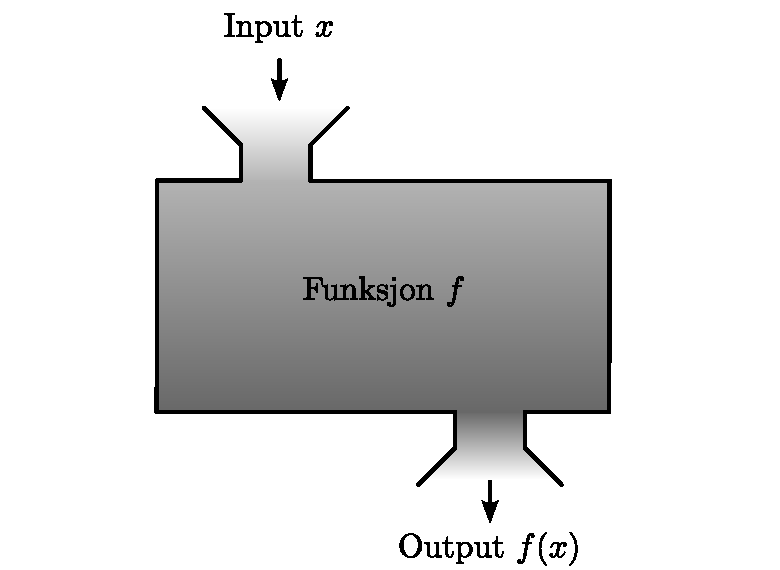
\includegraphics[width=0.8\textwidth]{function_blackbox}    
% \end{center}

% Hvis vi for eksempel ser på den matematiske funksjonen
% $$f(x) = x^2 + 3x + 1.$$
% Så kan vi for hver verdi av $x$ (input) beregne en resulterende verdi av $f(x)$ (output). Med andre ord er funksjonen $f$ en slags regel, eller maskin, som behandler et tall vi gir den. Vi kan definere denne funksjonen i Python som følger
% \begin{lstlisting}
% def f(x):
%     return x**2 + 3*x + 1    
% \end{lstlisting}
% \vspace{-0.3cm}
% her er \verb+def+ og \verb+return+ Python-kommandoer som vi skal forklare litt mer i detalj snart. Kort fortalt definerer vi her at det skal finnes en funksjon som heter $f$, som tar et tall $x$ inn, og gir tilbake (returnerer) tallet $f(x)$. Vi kan bruke funksjonen, vi kaller dette gjerne å "kalle på funksjonen", som følger
% \begin{lstlisting}
% print f(2)
% print f(3.5)
% print f(-1) + f(1)
% \end{lstlisting}
% \vspace{-0.3cm}
% som gir:
% \begin{lstlisting}
% 11
% 23.75
% 4
% \end{lstlisting}
% \vspace{-0.3cm}
% Så fort vi har definert en funksjon i python, huskes denne helt til programmet er ferdig å kjøre, og vi kan bruke den så mye vi ønsker. Funksjoner vi definerer, er egentlig bare en ny type variabel.

% En funksjon i python, trenger ikke nødvendigvis å være matematisk. Vi kan for-eksempel lage en funksjon som følger
% \begin{lstlisting}
% def greet(name):
%     print "Hello " + name + "!"
% \end{lstlisting}
% \vspace{-0.3cm}
% Denne funksjonen tar et navn som input, det vil si, en tekst-streng, og skriver ut en hilsen som output. Kommandoen
% \begin{lstlisting}
% greet("Lucy")
% \end{lstlisting}
% \vspace{-0.3cm}
% resulterer altså i
% \begin{lstlisting}
% Hello Lucy!
% \end{lstlisting}
% \vspace{-0.3cm}
% Merk at denne funksjonen ikke brukte kodenavnet \verb+return+, og når vi kallet på funksjonen, skrev vi ikke \verb+print+ før funksjonskallet. Dette er fordi funksjonen i seg selv printet, det var det vi hadde \emph{definert} at den skulle gjøre. Det er kanskje litt vanskelig å skjønne denne forskjellen, så la oss se på et par eksempler til.

% Vi definerer to funksjoner, $f_1$ og $f_2$. Vi vil at de begge skal ta et tall $x$ som input, og regne ut $2x$, altså det dobbelte. Forskjellen skal være at $f_1$ returnerer resultatet, mens $f_2$ printer det. Vi har altså:
% \begin{lstlisting}
% def f1(x):
%     return 2*x

% def f2(x):
%     print 2*x
% \end{lstlisting}
% \vspace{-0.3cm}
% La oss nå prøve å kalle på $f_1$ og $f_2$ på forskjellige måter og prøve å forstå hva som skjer. Først skriver vi:
% \begin{lstlisting}
% f1(2)
% \end{lstlisting}
% \vspace{-0.3cm}
% Vi får ikke noen feilmelding, så det virker greit. Men vi får heller ingen utskrift, det skjer ingenting! Dette er fordi vi kaller på $f_1$ med tallet 2 som input, funksjonen regner ut at $2*2 = 4$, og returnerer verdien, men så gjør vi ingenting med denne verdien. Vi kunne for eksempel gjort
% \begin{lstlisting}
% a = f1(2)
% print a
% \end{lstlisting}
% \vspace{-0.3cm}
% Her lagrer vi den returnerte verdien i en variabel \verb+a+, og så skriver vi ut \verb+a+. Nå får vi resultatet til skjerm, som er 4, flott!

% La oss nå prøve
% \begin{lstlisting}
% f2(3)
% \end{lstlisting}
% \vspace{-0.3cm}
% Dette fungerer veldig fint, vi får resultatet 6, rett til skjerm, flotte saker. Dette er fordi vi kaller på funksjonen $f_2$, som skriver tallet rett til skjermen. Om vi nå derimot prøver å lagre resultatet i en variabel
% \begin{lstlisting}
% a = f2(3)
% print a
% \end{lstlisting}
% \vspace{-0.3cm}
% får vi et litt mystisk resultat:
% \begin{lstlisting}
% 6
% None
% \end{lstlisting}
% \vspace{-0.3cm}
% For å skjønne hva som skjer her, så må vi først tolke kodelinjen \verb+a = f2(3)+, som vi lærte forrige uke, så betyr en slik linje at vi skal regne ut det som er på høyre-siden, og lagre det i variabelen \verb+a+. Vel, på høyre side kaller vi på $f_2$ med tallet $x=3$, $f_2$ gjør som vi har definert å skriver ut resultatet $2*x=6$ rett til skjerm. Etter det er $f_2$ ferdig, men den har ikke \emph{returnert} noen verdi, så når \verb+a+ settes lik resultatet på høyre-siden, så blir den ingenting, eller \verb+None+ som det heter i Python.

% Du har forhåpentligvis fått en viss idé om hva det nå betyr at en funksjon returnerer en verdi ved hjelp av \verb+return+-kommandoen. Ikke få panikk om du synes dette er ganske forvirrende, forståelse kommer med tid i programmering, så du skjønner det nok bedre etter du har fått prøvd deg litt frem!

% \subsection{Funksjoner av flere variabler}
% Når man først vet hvordan man lager funksjoner i python, er det superenkelt å lage funksjoner av flere variabler. Vi kan for eksempel lage følgende funksjon
% $$f(x,y) = 2x^2 + xy + 3,$$
% som følger
% \begin{lstlisting}
% def f(x,y):
%     return 2*x**2 + x*y + 3

% print f(3,4)
% \end{lstlisting}
% \vspace{-0.3cm}
% Tilsvarende kan vi lage funksjoner som ikke tar noen argumenter. Disse er kanskje mer nyttig i en programmeringssammenheng enn i en matematisk sammenheng. Vi kan foreksempel lage en funksjon
% \begin{lstlisting}
% def greet():
%     print "Hey there! I hope you have a great day!"
% \end{lstlisting}
% \vspace{-0.3cm}
% Merk at for å kalle på en slik funksjon, må vi fortsatt bruke parantesene, slik at et kall på \verb+greet+ skrives
% \begin{lstlisting}
% greet()
% \end{lstlisting}

% En ting det er verdt å merke seg er at mange av kommandoene vi har brukt i Python hitil, er funksjoner som er definert på akkurat den måten vi har lagt frem nå. For eksempel er \verb+range+ en funksjon, som vi kaller på når vi bruker. Når vi skriver; \verb+range(1,10,2)+ så gjør vi et funksjonskall med 3 inputtall.

% \clearpage

% \section{Arrays}

% Vi skal snart gå inn på plotting i Python, som vil si å lage figurer. Men da bør vi først nevne \verb+arrays+. Arrays er en spesiell type liste ment for matematikk. I motsetning til lister, som kan inneholde forskjellig type innhold, så kan arrays bare inneholde tall. Lister kan også gjøres større og mindre ved å legge til eller slette elementer, mens arrays \emph{alltid} har samme antall elementer. Om vi lager en array med tusen tall, så vil den arrayen alltid ha tusen tall, vi kan derimot endre hvilke tall den inneholder.

% Dere skal nå få se de to vanligste måtene å lage arrays på. Først, et tomt array. Ettersom at et array alltid har likt antall plasser, må vi spesifisere størrelsen på arrayet. Vi bruker kommandoen \verb+zeros+:
% \begin{lstlisting}
% x = zeros(3)    
% \end{lstlisting}
% \vspace{-0.3cm}
% Variabelen \verb+x+ er nå et array, med tre elementer. Der alle er satt til tallet 0. Dette virker kanskje litt rart å gjøre, men vi kan nå endre spesifikke elementer ved å indeksere på følgende måte
% \begin{lstlisting}
% x[0] = 10
% x[1] = 4
% x[2] = 3
% \end{lstlisting}
% \vspace{-0.3cm}
% Firkantparantesene kalles "indeksering", og brukes for å få tilgang til enkelt elementer av et array eller en liste. Python starter å telle på 0, så \verb+x[0]+ er det første elementet, og \verb+x[1]+ det andre, osv.
% Om vi nå skriver \verb+print x+ får vi nå resultatet
% \begin{lstlisting}
% [ 10.   4.   3.]
% \end{lstlisting}
% \vspace{-0.3cm}

% Neste måte lage et array på, er med funksjonen \verb+linspace+, som står for \emph{linear spacing}. Den tar tre inputparamtere: start, stop, antall.Om vi for eksempel skriver
% \begin{lstlisting}
% x = linspace(0,10,11)
% print x
% \end{lstlisting}
% \vspace{-0.3cm}
% får vi 
% \begin{lstlisting}
% [ 0.   0.2  0.4  0.6  0.8  1. ]
% \end{lstlisting}
% \vspace{-0.3cm}
% Altså er \verb+x+ et array med 6 elementer, hvor det første elementet er 0, det siste 1, og de resterende er jevnt fordelt. Vi kommer til å se at linspace er veldig praktisk når vi skal plotte.

% \subsection{Vektoriserte funksjoner}
% En stor fordel med arrays, er at de er laget for å drive med matematikk. Arrays oppfører seg foreksempel akkurat som vektorer. Det betyr at vi kan for eksempel bruke arrays til å regne prikkprodukt og kryssprodukt
% \begin{lstlisting}
% u = array([1,-4,3])
% v = array([3,2,-1])
% print dot(u,v)
% print cross(u,v)
% \end{lstlisting}
% \vspace{-0.3cm}
% \begin{lstlisting}
% -8
% [-2 10 14]
% \end{lstlisting}
% \vspace{-0.3cm}

% En annen veldig nyttig funksjonalitet, er at vi kan kalle på funksjoner med arrays som input, om vi for eksempel har laget funksjonen som vi så på tidligere
% \begin{lstlisting}
% def f(x):
%     return x**2 + 3*x + 1
% \end{lstlisting}
% \vspace{-0.3cm}
% så kan vi kalle på denne med et array som følger
% \begin{lstlisting}
% a = array([0,1,2,3,4,5])
% print f(a)
% \end{lstlisting}
% \vspace{-0.3cm}
% \begin{lstlisting}
% [ 1  5 11 19 29 41]
% \end{lstlisting}
% \vspace{-0.3cm}
% Det som skjer når vi kaller på funkjsonen med et array, er at Python regner ut resultatet element for element og returnerer et array med resultatene tilbake.

% \section{Plotting}
% Vi skal nå se på plotting i Python, som vil si å lage enkle figurer og grafer. Vi kommer til å tegne inn grafen vår i et koordinatsystem som vi er vant med fra matematikk. For å plotte bruker vi funksjonen \verb+plot+ fra pakken Pylab, som tar som input to lister, eller arrays, av tall. Vi kan altså for eksempel skrive
% \begin{lstlisting}
% plot([0,0.5,1], [2,4,6], 'x')
% show()
% \end{lstlisting}
% \vspace{-0.3cm}
% Her tegnes altså punktene (0,2), (0.5,4) og (1,6) inn i koordinatsystemet.
% Vi må bruke kommandoen \verb+show()+ for å vise figurer vi har laget. Vi har også lagt inn tekstrengen \verb+'x'+ i plotte-kommandoen, det er for at den skal tenge punktene vi gir som kryss. Hvis vi ikke ber den tegne kryss, tegner den rett og slett rette streker mellom punktene.

% Om vi har definert en funksjon, for eksempel:
% $$f(x) = x^2 + 3x + 1,$$
% som vi har sett på tidligere. Kan vi nå gjøre som følger
% \begin{lstlisting}
% def f(x):
%     return x**2 + 3*x + 1

% x = linspace(-6,6,1000)
% y = f(x)

% plot(x,y)
% show()
% \end{lstlisting}
% \vspace{-0.3cm}
% Her lager vi altså et sett med tusen punkter, som vi så plotter. Vi får dermed en fin figur av funksjonen $f(x)$. 

% Tilsvarende kan vi lage plot av velkjente matematiske funksjoner, for eksempel sinus og cosinus.
% \begin{lstlisting}
% x = linspace(0,2*pi,1000)
% plot(x,sin(x))
% plot(x,cos(x))
% show()
% \end{lstlisting}
% \vspace{-0.3cm}
% Merk at siden vi ga to plotte kommandoer før vi brukte show, så får vi to kurver i samme figur.

% Etter vi har lagd kurven ved å bruke \verb+plot+-kommandoen, og før vi bruker \verb+show+, så kan vi pynte på figuren vår. Vi kan for eksempel legge til navn på akser med
% \begin{lstlisting}
% xlabel('x')
% ylabel('y')
% \end{lstlisting}
% \vspace{-0.3cm}
% Vi kan lage tittel på figuren med \verb+title+-funksjonen på samme måte. Vi kan definere hvilke deler av figuren vi skal vise med \verb+axis+, for eksmepel
% \begin{lstlisting}
% axis([0,2*pi,-1,1])
% \end{lstlisting}
% \vspace{-0.3cm}
% vi gir altså en liste med \verb+[xstart, xstop, ystart, ystop]+.

% Vi kan også lagre figuren vår med
% \begin{lstlisting}
% savefig('figure1.png')
% savefig('figure1.pdf')
% \end{lstlisting}
% \vspace{-0.3cm}
% som lagrer bilde som filene 'figure1.png' og 'figure2.pdf' henholdsvis.

% Det er mange andre muligheter for å pynte på plot og få dem til å se kule ut, men la oss ikke dykke for dypt inn i det akkurat nå. Vi kommer til å se mer på plotte-muligheter iløpet av ukene som kommer, men om du er utålmodig kan du se på \url{matplotlib.org} som er nettsiden til plottepakken som pylab bruker, der finnes det mange eksempler på plots man kan lage.



% \clearpage


% \section*{Oppgave 1}
% \begin{itemize}
% \item[(a)] Definer en funksjon \verb+celsius_to_fahrenheit+ som tar grader $C$ som input, og returnerer grader Fahrenheit. Vi minner om at formelen for omregningen er
% $$F = \frac{9}{5}C + 32.$$
% \item[(b)] Bruk funksjonen til å finne ut hvor mange grader Fahrenheit disse tempraturene er: $20^\circ$, $0^\circ$, $-40^\circ$. 
% \item[(c)] Skriv en løkke der du lar gradier i Celsius gå fra -100 til 100 og skriv ut de tilhørende gradene i Fahrenheit ved å bruke funksjonen din. \\ \textbf{Hint 1:} Bruk \texttt{range}-funksjonen \\
% \textbf{Hint 2:} Du må kalle på funksjonen din inne i løkka.
% \end{itemize}


% \section*{Oppgave 2}
% Vi skal nå bruke løkker og \verb+range+-funksjonen til å regne ut noen matematiske summer
% \begin{itemize}
%     \item[(a)] Regn ut summen av alle oddetall under 1000.
%     \item[(b)] Regn ut summen av alle kvadrattall til og med 10000. \\ \textbf{Hint:} Vi er altså ute etter summen
%     $$1 + 4 + 9 + 16 + \ldots + 10000 = \sum_{i=1}^{100} i^2.$$
%     \item[(c)] Regn ut summen av den uendelige rekka
%     $$1 + \frac{1}{2} + \frac{1}{4} + \frac{1}{8} + \ldots$$
%     \textbf{Hint:} Hvert ledd i summen blir mindre og mindre, det holder altså å ta med for eksempel de 1000 første leddene. Da alle ledd etter dette vil bidra ekstremt lite til det endelige svaret
% \end{itemize}

% \section*{Oppgave 3}
% \begin{itemize}
%     \item[(a)] Plot $e^x$ for $x\in[0,2]$.
%     \item[(b)] Lag et plot, der du viser de tre funksjonene:
%     $$e^x, \qquad e^{-x}, \qquad 1/e^{x}.$$
%     for $x \in [0,2]$. Her må du bruke \verb+axis+-kommandoen for å velge rimelige akser på figuren din!
%     \item[(c)] Pynt på plottet du nettopp lagde ved hjelp av funksjonene \verb+axis+, \verb+xlabel+, \verb+legend+, \verb+title+ og \verb+grid+.
%     \item[(d)] Lagre plottet ditt som en .pdf-fil, og som en .png-fil. Sjekk at filene ble lagret riktig og at de ser ut som forventet.
% \end{itemize}



% \clearpage

% \section*{Utfordringer!}
% \subsection*{Primtall}
% Greier du å skrive en funksjon som tar et heltall som input, og finner ut om det er et primtall eller ikke?
% \subsection*{Fibonacci}
% Greier du å skrive et program som regner ut og skriver ut Fibonacci-tallene?
% \subsection*{Project Euler}
% På nettsiden \url{www.projecteuler.net} er det mange morsomme matematiske nøtter som er ment å løses ved programmering. Se om du greier å få til et par av de første oppgavene. Spør gjerne om hjelp.


% Denne uken kommer hovedsakelig til å gå med til repetisjon av tidligere programmering, for den delen er det greit å se på notatene fra forrige gang, samt å se på oppgavene vi har gitt dere der.

% Andre halvdel av denne uka kommer til å gå med til å starte å se på fysikken vi skal løse i de siste to ukene av prosjektet, og det er det vi skriver om i dette notatet.


% \section{Fallskjermhopping}

% Vi skal nå begynne å studere hvordan hastigheten til en person som hopper i fallskjerm endrer seg over tid. Vi kommer til å finne matematiske ligninger basert på vår fysiske forståelse av de kreftene som virker på hopperen. Vi skal diskutere ligningene vi kommer frem til, og se på hvorfor ikke greier å løse dem med kun penn og papir. Vi skal derfor se hvordan vi kan løse ligningene ved hjelp av programmering.


% Et fallskjermhopp består hovedsakelig av to deler. Den første delen er det som skjer før fallskjerm er utløst, denne delen kalles gjerne \emph{fritt fall}, i de fleste sportssammenhenger vil man oppleve ca ett minutt fritt fall per hopp. Etter dette utløser hopperen fallskjermen som da drastisk reduserer fallhastigheten, under fallskjerm brukeren hopperen så vanligvis fra ett til tre minutter videre ned til bakken avhengig av hvor stor fallskjerm de bruker og hvor nærme bakken de utløste skjermen.

% I begge faser utsettes hopperen bare for to krefer, tyngdekraft og luftmotstand. Så vi har
% $$\sum F = F_G + F_D,$$
% der $F_G$ er tyngdekraften og $F_D$ er luftmotstand. Dere har sikkert kjennskap til at tyngdekraften er gitt ved
% $F_G = mg,$
% der $m$ er den totale massen til hopperen, som vil se personvekten og alt utstyret, og $g$ er tyngdens akselersjonskonstant, som vi setter til $g=9.81$ m/s$^2$. En fallskjermhopper vil falle med veldig høy hastighet, og vi bruker derfor en kvadratisk form på luftmotstanden, som vi kan skrive som følger
% $$F_D = \frac{1}{2}\rho C A v^2,$$
% her er $\rho$ tettheten til luft, $C$ er luftmotstandskoeffisienten som avhenger av formen på objektet som faller og $A$ er frontarealet.
% For å slippe å skrive så mye kaller vi disse tallene samlet for $D$, slik at
% $$\frac{1}{2}\rho C A = D,$$
% $$F_D = -Dv^2.$$
% ligningen vi skal løse har altså følgende form
% $$ma = mg - D v^2.$$
% Dette er det som matematisk kalles en differensialligning, la oss diskutere hva det betyr.

% \section*{Differensialligninger}
% Tidligere når vi har sett på ligninger, så er det et matematisk uttrykk, der vi løser for en ukjent. For eksempel kan vi ha ligningen
% $$x^2 + 7 = 56.$$
% Dette er en ligning fordi vi har en "likhet". Og vi vet at vi kan løse denne for $x$, ved å flytt over konstanten $7$, og så ta roten, da finner vi at 
% $$x = \pm 7.$$
% Altså har vi løst ligningen, og funnet at $x$ er 7. En differnsialligning er også en ligning fordi den innholder en "likhet" på samme måte, og den har en ukjent vi løser for. Den store forskjellen er at den ukjente vi løser for, er ikke lenger et enkelt tall, men det er derimot en funksjon.

% Newtons 2.\ lov er et perfekt eksempel på en differensialligning, som vi løser for å finne enten farten, eller posisjonen, til et objekt. Her er både farten, og posisjonen, eksempler på funksjoner, fordi de endrer seg med tid: $v(t)$, $x(t)$. En differensialligning vil innholde den deriverte av funksjonen vi er ute etter, som er mer synlig om vi skriver akselerasjonen som den deriverte av hastigheten i Newtons 2.\ lov:
% $$\sum F = ma = m\frac{\d v}{\d t}.$$
% Differensialligningen vi prøver å løse er:
% $$m\frac{\d v}{\d t} = mg - D v(t)^2.$$

% Så, hvordan løser vi en slik ligning? Vel, det finnes utrolig mange forskjellige typer differensialligninger, og det finnes enda flere metoder før å løse dem! De som tar R2, kommer til å lære en del om å løse denne type ligninger, men vi har ikke tid til å dekke så altfor mye av det pensumet her.

% \subsection*{Uløslighet}
% Differensialligningen vi ønsker å løse er
% $$m\frac{\d v}{\d t} = mg - D v(t)^2,$$
% og vi ønsker å løse den for hastigheten $v(t)$. Men dette får vi ikke til, fordi akselerasjonen avhenger av hastigheten. Dette er nettopp grunnen til at vi ofte ser bortifra luftmotstand når vi løser Newtons 2.\ lov. Ofte er dette greit fordi resultatet er tilnærmet likt med og uten. Men, i visse tilfeller vil luftmotstand gi et veldig stort forskjell - og det er tilfellet i fallskjermhopping.

% \section{Fremgangsmåte}
% Så, hvordan kan vi løse en uløselig ligning ved hjelp av programmering? Idéen er ganske enkel, men la oss prøve å ta det steg for steg.

% La oss starte med å se på hvordan det hadde gått om vi hadde sett bortifra luftmotstand, da hadde vi hatt fritt fall
% $$ma = \sum F = mg,$$
% slik at akselerasjonen hadde vært konstant
% $$a = g.$$
% I det tilfellet hadde vi kunnet bruke bevegelsesligningene, som hadde gitt oss svarene
% $$v(t) = v_0 + at.$$
% og 
% $$x(t) = x_0 + v_0 t + \frac{1}{2}at^2.$$
% Altså ser vi at hastigheten vokser konstant for alltid. Som selvfølgelig ikke kan stemme, da vi vet at en fallskjermhopper vil treffe \emph{terminalhastighet} ganske fort.

% \subsubsection*{Terminalhastighet}
% Terminalhastigheten er den raskeste hastigheten et objekt kan falle med, og vi kan enkelt finne den uten å løse differensialligningene vår, vi vet at når luftmotstanden er like stor som tyngdekraften, så vil summen av kreftene på hopperen være 0, og da er akselerasjonen null og falleren faller med en konstant hastighet, nemlig terminalhastigheten. Vi har altså
% $$mg = \frac{1}{2}\rho C A v_T^2,$$
% når vi løser denne for terminalhastigheten har vi
% $$v_T = \sqrt{\frac{2mg}{\rho C A}},$$
% og når vi setter inn rimelige verdier ($m=90$ kg, $C=1.4$, $\rho=1$ kg/m$^3$, $A=0.7$ m$^2$, $g=9.81$ m/s$^2$) får vi
% $$v_T = 42.4 {\rm\ m/s} = 153 {\rm\ km/h}.$$

% \section{Bruke bevegelsesligningene med luftmotstand}
% Om vi nå legger til luftmotstanden igjen, vet vi at vi ikke kan bruke bevegelsesligningene, fordi vi ikke har konstant akselerasjon. Vi har
% $$a(v) = g - \frac{1}{2m}Dv^2,$$
% og ettersom at hastigheten øker, så vil akselerasjonen minke med tiden. Merk at vi skriver $a(v)$, fordi akselerasjonen er en funksjon av hastigheten. Om vi derimot ser på en veldig liten tidsendring $\Delta t$, så vet vi at hastigheten vil endre seg veldig lite, så vi kan bruke bevegelsesligningene et kort \emph{steg} frem i tid ved å si at akselerasjonen er konstant en kort tid:
% $$v_1 = v_0 + a(v_0)\Delta t.$$
% Nå har vi altså funnet hastigheten til hopperen en kort tid etter han startet. Vi kan nå gå enda litt lenger frem i tid, ved å oppdatere akselerasjonen, og si at den er konstant en ny kort tidsperiode
% $$v_2 = v_1 + a(v_1)\Delta t.$$
% Trikset her, er å la $\Delta t$ være veldig liten, slik at akselerasjonen er tilnærmet konstant. Vi må derfor ta veldig mange slike små tidsteg:
% $$v_{n+1} = v_n + a(t_n)\Delta t,$$
% og på denne måten kan vi løse differensialligningen vår et skritt av gangen til vi har funnet hele løsningen.

% \subsection{En mer matematisk tankemåte}
% Differensialligningen vår er
% $$a = g - \frac{D}{m}v^2,$$
% og vi kan skrive akselerasjonen som den deriverte av hastigheten
% $$\frac{\d v}{\d t} = g - \frac{D}{m}v^2.$$
% Definisjonen av den deriverte av $v$ er
% $$a = \frac{\d v}{\d t} = \lim_{\Delta t \to 0} \frac{v(t+\Delta t)-v(t)}{\Delta t}.$$
% Vi kan si at vi tilnærmer den deriverte ved istedenfor å la $\Delta t$ gå helt mot 0, at vi stopper den på et lite tall, vi har da at
% $$a = \frac{\d v}{\d t} \approx \frac{v(t+\Delta t) - v(t)}{\Delta t}.$$
% slik at
% $$v(t+\Delta t) = v(t) + a\Delta t.$$
% Vi ser altså at dersom vi kjenner farten ved tiden $t$, så kan vi finne den en kort tid senere ved å plusse på $a \Delta t$, der vi kan "late som" akselerasjonen er konstant.



% Vi er nå klare for å trekke sammen alle trådene vi har sett på så langt og begynne å lage et program som løser bevegelsesligningene for fallskjermhopping og strikkhopp. Vi starter med litt repetisjon av fysikken, og så ser vi på hvordan vi skal implementere det på datamaskin.


% \section*{Kreftene}


% Et fallskjermhopp består hovedsakelig av to deler. Den første delen er det som skjer før fallskjerm er utløst, denne delen kalles gjerne \emph{fritt fall}. Etter dette utløser hopperen fallskjermen som da drastisk reduserer fallhastigheten. I begge faser utsettes hopperen bare for to krefer, tyngdekraft og luftmotstand. Så vi har
% $$\sum F = F_G + F_D,$$
% der $F_G$ er tyngdekraften og $F_D$ er luftmotstand. Dere har sikkert kjennskap til at tyngdekraften er gitt ved
% $F_G = mg,$
% der $m$ er den totale massen til hopperen, som vil se personvekten og alt utstyret, og $g$ er tyngdens akselersjonskonstant.  En fallskjermhopper vil falle med veldig høy hastighet, og vi bruker derfor en kvadratisk form på luftmotstanden, som vi kan skrive som følger
% $$F_D = \frac{1}{2}\rho C A v^2,$$
% her er $\rho$ tettheten til luft, $C$ er luftmotstandskoeffisienten som avhenger av formen på objektet som faller og $A$ er frontarealet.

% Det eneste som endrer seg når fallskjerm løses ut, er frontarealet $A$, og luftmotstandskoeffisienten $C$. Ellers er fysikken helt lik.

% \subsection*{Parametere}
% Tallene $m$, $g$, $\rho$, $C$, $A$ er det som kalles fysiske parametere, og det er størrelser vi velger - vi velger dem utifra hva slags simulering vi ønsker å gjøre, men vi regner dem altså generelt sett som kjent. I vår simulering kan vi bruke følgende parametere
% \begin{center}
% \begin{tabular}{c|c}
% Fritt Fall \\ \hline
% $m$ & 90 kg \\ \hline
% $g$ & 9.81 m/s$^2$ \\ \hline
% $\rho$ & 1 kg/m$^3$\\ \hline
% $C$ & 1.4 \\ \hline
% $A$ & 0.7 m$^2$\\ \hline \hline
% Under fallskjerm \\ \hline
% $C_{\rm p}$ & 1.8 \\ \hline
% $A_{\rm p}$ & 44 m$^2$
% \end{tabular}
% \end{center}

% \subsection*{Newtons 2.\ lov}

% Om vi bruker Newtons 2.\ lov sammen våre kraftlover får vi et uttrykk fra akselerasjonen til fallskjermhopperen. Vi har:
% $$\sum F = ma,$$
% setter vi inn kreftene får vi
% $$F_g + F_d = ma,$$
% da har vi
% $$mg - \frac{1}{2}\rho C A v^2 = ma,$$
% vi deler på $m$ for å få et uttrykk for $a$:
% $$a = g - \frac{1}{2m}\rho C A v^2.$$
% Vi ser at akselerasjonen avhenger av hastigheten, så vi kan skrive den som en funksjon av $v$:
% $$a(v) = g - \frac{1}{2m}\rho C A v^2.$$

% \section*{Oppgave - Regne ut terminalhastigheten}
% Terminalhastigheten er den raskeste hastigheten et objekt kan falle med. Regn ut terminalhastigheten for fallskjermhopperen vi ser på. \\ 
% \textbf{Hint:} Ved terminalhastigheten faller man med konstant hastighet, da vet vi at akselerasjonen er null. Hva betyr dette med tanke på Newtons 2.\ lov?

% \clearpage

% \section*{Fremgangsmåte for å finne hastigheten til hopperen}
% Vi vet at dersom vi har en konstant akselerasjon, og en starthastighet $v_0$ så kan vi regne ut hastigheten ved en hvilken som helst tid $t$ utifra:
% $$v(t) = v_0 + at, \qquad \mbox{for konstant } a.$$
% Så hva gjør vi når vi \emph{ikke} har en konstant akselerasjon? I vårt tilfelle vil akselerasjonen endre seg over tid, fordi hastigheten endrer seg over tid. Men over en veldig kort tid $\Delta t$, så kan vi si at den er så godt som konstant, vi kan da si at
% $$v_1 = v_0 + a(v_0) \Delta t.$$
% Der $v_0$ er starthastigheten, $v_1$ er hastigheten etter ett \emph{tidssteg}, 
% altsa ved tiden $t_1 = \Delta t$.
% Vi skriver $a(t_0)$ for å tydliggjøre at vi bruker akselerasjonen som gjelder
%  ved starttiden. Siden vi nå kjenner $v_1$, så kan vi regne ut $a(v_1)$ fra uttrykket vårt for akselerasjonen, og bruke denne til å gå et tidssteg til:
% $$v_2 = v_1 + a(v_1) \Delta t.$$
% Og slik kan vi fortsette, vi kan alltid regne oss ett tidssteg frem, ved å bruke resultatet fra forrige tidssteg
% $$v_{n+1} = v_n + a(v_n)\Delta t,$$
% for $n=0,1,2,3,\ldots$.

% Slik fortsetter vi til vi har simulert nok tidssteg til å nå en slutttid vi har valgt på forhånd. Vi ønsker gjerne at $\Delta t$ skal være minst mulig, slik at vi får et mer nøyaktig resultat. For eksempel kan vi bruke $\Delta t = 0.01$ s i vår simulering, altså tar vi skritt på ett hundredelssekund frem i tid av gangen. I et vanlig fallskjermhopp er hopperen ca.\ 1 minutt i fritt fall, så vi lar sluttiden være $T=60$ sekunder. Det betyr at vi trenger å ta totalt
% $$n = \frac{T}{dt} = \frac{60 \mbox{ s}}{0.01 \mbox{ s}} = 6000,$$
% tidssteg.

% \clearpage 

% \section*{På tide å programmere}

% Vi er nå klare for å sette igang, her er malen på programmet dere kommer til å skrive:
% \begin{itemize}
%     \item[1] Importer pylab, det er alt vi kommer til å trenge.
%     \item[2] Skriv inn alle parameterene vi trenger, det vil si $m$, $g$, $\rho$, $A$, $C$, $A_{p}$, $C_{\rm p}$, $v_0$.
%     \item[3] Definer akselerasjonen som en funksjon av hastigheten. \\
%     \textbf{Hint:} \verb+def a(v):+, og husk å returnere noe!
%     \item[4] Definer $\Delta t = 0.01$ (Hint: kall variablen \verb+dt+ i programmet ditt), $T=60$ og $n = T/dt$
%     \item[5] Opprett to \emph{arrays}, ett for hastigheten $v$ og et for tiden $t$. Vi vil at de skal være tomme, og ha plass til $n+1$ elementer, så bruk \verb+zeros+ kommandoen. Merk at nå vil \verb+v[i]+ i programmet ditt svare til $v_i$ i matematikken.
%     \item[6] Lag en \verb+for+-løkke som går over $i=0,1,2,\ldots,n$. (Hint, bruk \verb+range+.)
%     \item[7] Inne i løkka, regn ut $v[i+1]$ fra $v[i]$ ved å bruke formelen vi har funnet. Oppdater også tiden (Hint: \verb!t[i+1] = t[i] + dt!).
%     \item[8] Plot resultatet for å sjekke at alt har blitt gjort riktig (Hint: \verb+plot(t,v)+).
% \end{itemize}

% \section*{Oppgaver}
% Etter at du har fått programmet ditt til å funke kan du besvare følgende oppgaver
% \begin{itemize}
%     \item[a)] Pynt på plottet ved å lagge til navn på aksene (\verb+xlabel+ og \verb+ylabel+), et grid (\verb+grid()+) og eventuelt tittel og lignende.
%     \item[b)] Hvor lang tid tar det før falleren har nådd tilnærmet terminalhastighet? Les av plottet.
%     \item[c)] Skriv ut terminalhastigheten hopperen får i programmet ditt. Hint: Det er en funksjon \verb+max+, som henter ut det største elementet i et array. Sammenlign denne med terminalhastigheten du fant med penn og papir tidligere, hvor like blir verdiene? Ser det ut som programmet ditt regner riktig?
% \end{itemize}

% \clearpage

% \section*{Videre}
% Nå har vi laget et program, som finner hastigheten til hopperen under fritt fall med luftmotstand. Men vi må fortsatt legge til at fallskjerm utløses. Vi kommer til å se på dette i fellesskap neste gang, men de av dere som har fått til alt så langt, kan begynne å bryne dere på hvordan vi skal gjøre dette. Grunnidéen er ihvertfall denne: det er bare frontarealet $A$ og luftmotstandskoeffisienten $C$ som endrer seg når fallskjerm løses ut, så hvis vi greier å endre disse verdiene i programmet vårt til riktig tidspunkt, så simulerer vi effektivt at fallskjerm er løst ut. I løkka vår, så har vi tiden $t_i$, så kanskje vi greier å bruke en \verb+if+-test til å endre $A$ og $C$ til riktig tid?

% Neste gang kommer vi også til å regne ut og plotte $g$-kreftene fallskjermhopperen opplever. Vi kommer også til å finne hastigheten til en strikkhopper på samme måte som vi har gjort for fallskjermhopperen idag.


% Sist uke laget vi et program som løste bevegelsesligningene for fallskjermhopping. Vi startet med Newtons 2.\ lov, og så på kreftene som virket. Fra dette fant vi et uttrykk for akselerasjonen, og vi brukte så bevegelsesligningene vi vent gjelder ved konstant akselerasjon til å løse for hastigheten små steg fremover i tid.

% Idag skal vi gjøre det samme for posisjon, og vi skal da se på strikkhopp som et eksempel. Når vi ser på strikkhopp, er det egentlig bare uttrykket for akselerasjon som endrer seg, alt annet kan være helt likt. Men ettersom at kreftene som virker på en strikkhopper avhenger av posisjonen til hopperen, må vi også løse for posisjonen.

% Etter vi har sett på det kommer vi til å plott $g$-kreftene både for fallskjerm- og strikkhopperen. Vi kan da sammenligne strikk og fallskjermhopp baser på $g$-kreftene hopperen føler. Vi kommer også til å se på hvordan fallskjermen løses ut, og hvordan det påvirker $g$-kreftene hopperen utsettes for.

% \clearpage

% \section*{Å løse for posisjon}
% Sist uke fant vi først et uttrykk for akselerasjonen for en fallskjermhopper som var
% $$a(v) = g - \frac{1}{2}C\rho A v^2.$$
% og vi brukte så bevegelsesligningene som gjelder ved konstant akselerasjon
% $$v = v_0 + a t,$$
% til å ta små "tidssteg" på $\Delta t$, som ga oss
% \begin{align*}
% v_1 &= v_0 + a(v_0)\Delta t \\  
% v_2 &= v_1 + a(v_1)\Delta t \\
% v_3 &= v_2 + a(v_2)\Delta t \\
% &\hdots \\
% v_{i+1} &= v_i + a(v_i)\Delta t.
% \end{align*}

% Vi har også en bevegelsesligning ved konstant akselerasjon som gjelder for posisjon
% $$x = x_0 + v_0 t + \frac{1}{2}at^2,$$
% vi kan bruke denne til å ta "tidssteg" på samme måte som for hastigheten
% \begin{align*}
% x_1 &= x_0  + v_0 \Delta t + \frac{1}{2} a(v_0) \Delta t^2 \\  
% x_2 &= x_1  + v_1 \Delta t + \frac{1}{2} a(v_1) \Delta t^2 \\  
% x_3 &= x_2  + v_2 \Delta t + \frac{1}{2} a(v_2) \Delta t^2 \\  
% &\hdots \\
% x_{i+1} &= x_i + v_i\Delta t + \frac{1}{2} a(v_i)\Delta t^2.
% \end{align*}

% \clearpage

% \section*{Strikkhopp}
% La oss nå se på en strikkhopper og kreftene som virker på henne. Vi kan tenke på strikken som en slags fjær når den er strukket ut. Men når strikken er "trykket" sammen gir den ingen kraft (i motsetning til en fjær, som virker "begge veier"). Når hopperen hopper fra toppen av en bru, er strikken slynget sammen, og kommer derfor ikke til å påvirke hopperen før hun har falt langt nok til at strikken begynner å bli strukket ut.  Vi kaller punktet der strikken akkurat ikke er begynnt å bli strukket ut for likevektspunktet.

% La oss nå lage et referansesystem som passer bra til problemet vi ser på. Vi plasserer $x=0$ i likevektspunktet. Vi sier at strikken er 20 meter lang, så hopperen hopper fra et punkt som er 20 meter høyere enn likevektspunktet, altså i $x_0 = 20$ m. La oss også si at det går en elv under brua, og at brua er 60 m over elva.

% \begin{figure}[h!b]
% \centering
% 
\includegraphics[width=0.9\textwidth]{Bungee_bridge}
% \end{figure}

% Vi ser nå at dersom posisjonen til hopperen er over likevektspunktet, så vil strikken ikke være strukket ut, og den virker ikke med noen kraft på hopperen. Siden vi har plassert likevektspunktet i $x=0$, betyr dette at strikkraften, som vi vil kalle $S$, er 0 hvis $x>0$.

% Hvis $x<0$ derimot, ser vi at strikken er strukket ut, og vil dermed trekke hopperen oppover med en fjærkraft. Denne fjærkraften modellerer vi med det som kalles Hooke's lov, som sier at kraften fra en fjær som er strukket ut en lengde $x$ er gitt ved:
% $$F = -kx,$$
% der $k$ er fjærstivheten. 

% Vi kan altså uttrykke den kraften fra strikken som en funksjon av posisjonen $x$ som følger:
% $$S(x) = \begin{cases} 0 & \mbox{hvis } x>0 \\
% -kx & \mbox{hvis } x \leq 0
% \end{cases}.$$

% I tilegg til snorkraften $S(x)$, virker det en tyngdekraft $mg$, og en luftmotstand $Dv$, på hopperen. Fra Newtons 2.\ lov
% $$\sum F = ma,$$
% har vi da
% $$S(x) - mg - Dv = ma.$$
% Vi løser for akselerasjonen, som vi nå ser er en funksjon av både posisjon og hastighet:
% $$a(x,v) = \frac{S(x)}{m} - g - \frac{D}{m}v.$$

% Ettersom at akselerasjon nå er en funksjon av både hastighet og posisjon, må vi løse for hastighet og posisjon samtidig, så vi har
% \begin{align*}
% v_1 &= v_0 + a(x_0, v_0)\Delta t \\
% x_1 &= x_0 + v_0\Delta t + \frac{1}{2}a(x_0, v_0)\Delta t^2 \\
% v_2 &= v_1 + a(x_1, v_1)\Delta t \\
% x_2 &= x_1 + v_1\Delta t + \frac{1}{2}a(x_1, v_1)\Delta t^2 \\
% &\hdots \\
% v_{i+1} &= v_i + a(x_i, v_i)\Delta t \\
% x_{i+1} &= x_i + v_i\Delta t + \frac{1}{2}a(x_i, v_i)\Delta t^2 \\
% \end{align*}

% \clearpage

% \section*{Kode strikkhopp}
% Du skal nå endre programmet du skrev sist uke til å løse for strikkhopping. Her er malen på hva programmet skal inneholde
% \begin{enumerate}
%     \item Importer pylab, det er alt vi kommer til å trenge.
%     \item Skriv inn alle parameterene vi trenger. Bruk $m=60$, $v_0=0$, $x_0=20$, $D=10$. Gjett på en verdi for fjærstivheten $k$, vi kommer til å justere den etterhvert.
%     \item Definer snorkraften $S(x)$. Her må du bruke \verb+def+ til å definere en funksjon, og en \verb+if+-test inne i funksjonen for å sjekke om $x>0$ eller $x<=0$. 
%     \item Definer akselerasjonen som funksjon av både posisjon og hastighet. \verb+def a(x,v):+.
%     \item Definer $\Delta t = 0.01$ (Hint: kall variablen \verb+dt+ i programmet ditt), $T=60$ og $n = T/dt$
%     \item Opprett tre \emph{arrays}, ett for hastigheten $v$, ett for posisjonen $x$ og ett for tiden $t$. Vi vil at de skal være tomme, og ha plass til $n+1$ elementer, så bruk \verb+zeros+ kommandoen. 
%     \item Sett første element i $x$-arrayet til å være $x_0$. Altså \verb+x[0] = x0+.
%     \item Lag en \verb+for+-løkke som går over $i=0,1,2,\ldots,n$. (Hint, bruk \verb+range+.)
%     \item Inne i løkka, regn ut $t[i+1]$, $v[i+1]$ og $x[i+1]$. Fra de følgende formlene
%     \begin{align*}
%     t_{i+1} &= t_i + \Delta t, \\
%     v_{i+1} &= v_i + a(x_i, v_i)\Delta t, \\
%     x_{i+1} &= x_i + v_i\Delta t + \frac{1}{2}a(x_i, v_i)\Delta t^2.
%     \end{align*}
%     Vi har altså
%     \begin{lstlisting}
% for i in range(n):
%     t[i+1] = t[i] + ...
%     v[i+1] = v[i] + ...
%     x[i+1] = x[i] + ...    
%     \end{lstlisting}
%     \item Plot resultatet for å sjekke at alt har blitt gjort riktig (Hint: \verb+plot(t,x)+).
% \end{enumerate}

% \subsection*{Oppgave}
% \begin{itemize}
%     \item[a)] Pynt på plottet ditt. Sett navn på akser osv.
%     \item[b)] Ved å se på plottet, prøv å juster fjærstivheten $k$ sånn at hopperen akkurat rører vannet. Altså at bunnen av kurven akkurat når $-40.$
%     \item[c)] Skriv ut makshastigheten hopperen opplever. Hint: \verb+max(v)+. Hvordan er dette sammenlignet med makshastigheten til fallskjermhopperen?
% \end{itemize}

% \clearpage

% \section*{Plotte $g$-krefter}
% Begrepet $g$-kraft er noe misvisende, da det egentlig ikke er snakk om "krefter" man opplever - men akselerasjon. Når menneskekroppen blir akselerert, føler vi dette som vekt. Tenkt for eksempel når du sitter i en bil som kjører gjennom en sving, og du blir "dratt" til siden. Disse akselerasjonene føles altså ut som en slags kraft på kroppen, og det er derfor vi snakket om $g$-krefter. Bokstaven "g" i $g$-kraft står for gravitasjon, og det er fordi vi sammenligner den kraften en person med tyngdekraften. Når du står helt i ro, føler du $1g$ fra tyngdekraften. I en berg-og-dalbane vil man etterhvert som man følger banen oppleve mye forskjellige $g$-krefter etterhvert som man akselerer inn og ut av svinger og opp og ned bakker. Når vi har et hurtig dykk nedover på en berg-og-dalbane blir man vektløs, som altså er $0g$, eller fritt fall. En fordel med å snakke om $g$-krefter fremfor de faktiske fysiske kreftene som virker på et objekt, er at de ikke avhenger av massen. Alle personer vil altså kjenne de samme $g$-kreftene i den samme berg-og-dalbanen.

% For å regne ut $g$-kreftene hopperen føler i begge tilfeller trenger vi egentlig bare å legge til et nytt array i løkka, hvor vi regner ut akselerasjonen som virker på hopperen, deler på $g$ og legger til 1. Koden er som følger:
% \begin{lstlisting}
% gforces = zeros(N+1)
% ...


% for i in range(N):
%     t[i+1] = t[i] + ...
%     v[i+1] = v[i] + ...
%     x[i+1] = x[i] + ...
%     gforces[i] = a(x[i],v[i])/g + 1
% \end{lstlisting}

% \subsection*{Oppgave}
% Regn ut og plot $g$-kreftene som virker på både fallskjerm- og strikkhopperen i programmet ditt. Sammenlign plottene, er de forskjellige? Forklar så godt du kan hvorfor de to er forskjellige.

% \clearpage

% \section*{Utløse fallskjermen}
% Vi har nå kommet til tidspunktet der vi skal løse ut fallskjermen i programmet vårt. Vi har nevnt tidligere at det eneste vi egentlig trenger å gjøre er å endre luftmotstandskoeffisienten $C$ til $C_{\rm P} = 1.8$ og frontarealet $A$ til $A_{\rm p} = 44$. Vi har hitill simulert fallskjerm hopperen i $T=60$ sekunder, la oss øke denne tiden til 180 sekunder. Men vi lar fortsatt den første løkka bare gå over de første 60 sekundene, deretter endrer vi $C$ og $A$, og løser for de siste 120 sekundene, altså
% \begin{lstlisting}
% dt = 0.01
% T = 180
% n = int(T/dt)

% # Simuler de forste 60 sekundene
% for i in range(0, 60/dt):
%     t[i+1] = t[i] + dt
%     v[i+1] = v[i] + a(v[i])*dt
%     gforces[i] = 1 - a(v[i])/g

% # Endre C og A
% C = C_p
% A = A_p

% # Simuler de siste 120 sekundene
% for i in range(60/dt, 180/dt):
%     t[i+1] = t[i] + dt
%     v[i+1] = v[i] + a(v[i])*dt
%     gforces[i] = 1 - a(v[i])/g
% \end{lstlisting}

% Nå kan vi plotte både hastigheten mot tid, og $g$-kreftene. Hva ser vi da? Et problem vi har fått er at vi endrer verdiene av $C$ og $A$ altfor brått. Dette er altså som om fallskjermen hadde blitt utløst umiddelbart, som hadde bremset ned hopperen enorm fort, og fører til nesten 100 $g$! Alt over 10 $g$ kan være livsfarlig og de fleste vanlige personer begynner å besvime når man går over $5$g.

% Moderne fallskjermer er defor laget for å løse seg ut saktere med vilje, det gir dermed en roligere nedbremsning. La oss prøve å simulere at fallskjermen bruker 5 sekunder på å løse seg fullstendig ut, og se hvordan de påvirker $g$-kreftene. Vi lager nå tre løkker. En helt uten skjerm, en der fallskjermen er i prosessen å løse seg ut, og en der skjermen er helt løst ut.

% \begin{lstlisting}
% dt = 0.01
% T = 180
% n = int(T/dt)

% # Simuler de forste 60 sekundene
% for i in range(0, 60/dt):
%     t[i+1] = t[i] + dt
%     v[i+1] = v[i] + a(v[i])*dt
%     gforces[i] = 1 - a(v[i])/g

% # Simulerer de neste 5 sekundene
% for i in range(60/dt, 65/dt):
%     C += (C_p-C)/(5/dt)
%     A += (A_p-A)/(5/dt)

%     t[i+1] = t[i] + dt
%     v[i+1] = v[i] + a(v[i])*dt
%     gforces[i] = 1 - a(v[i])/g

% # Simuler de siste 115 sekundene
% for i in range(65/dt, 180/dt):
%     t[i+1] = t[i] + dt
%     v[i+1] = v[i] + a(v[i])*dt
%     gforces[i] = 1 - a(v[i])/g
% \end{lstlisting}



\end{document}


“Programs must be written for people to read, and only incidentally for machines to execute.” 

